%!TEX TS-program = xelatex
%!TEX encoding = UTF-8 Unicode
% !TEX root = ../../metp.tex
\begin{refsection}

\chapter{STEREOFONIA}
\startcontents[chapters]
\printcontents[chapters]{}{1}{}

\vfill\null

Il primo passo necessario verso la comprensione del concetto di \emph{Stereofonia},
per di arrivare alle tecniche ed alle tecnologie elettroacustiche che la
rendono possibile, è stabilire una base concettuale solida attraverso
l'etimologia del termine e dei termini ad esso collegati. \emph{Stereo}, dal greco
\emph{Stere\'os}, significa \emph{solido}. Non un numero, non una configurazione
ma un aggettivo qualitativo. Nel dizionario inglese Oxford: \emph{Solid, firm
and stable in shape. Having three dimensions}. Solido, \emph{solid}, dalla radice
latina di \emph{Solidus, Sollus}, intero.

Con la parola \emph{Stereofonia} dovremmo quindi descrivere una condizione
nella quale \emph{phon\={e}}, sempre dal greco, \emph{suono}, la \emph{voce},
arrivi all'ascoltatore solida, integra, ferma e stabile nella sua forma (sonora)
multi dimensionale, intera.

%\clearpage

Indispensabile, a questo punto, all'intera comprensione è anche la descrizione
del concetto di \emph{mono}, dal quale deriviamo il nomignolo \emph{monofonico},
espressione del legame tra \emph{monos}, \emph{solo, unico, costituito da uno solo}
e \emph{phon\={e}} (suono): un unico suono, una voce, \emph{one voice},
\emph{alone}, sola. Non siamo nuovi alla definizione di monofonia nei termini di
una sola voce in quanto la stessa parola è utilizzata nella descrizione
del canto gregoriano (ad una voce), successivamente evolutasi nella \emph{polifonia}
(dal greco \emph{poluph\={o}nia}, da \emph{polu}, molte e \emph{phon\={e}},
voci). La tradizionale dicotomia quindi, se proprio deve essercene una, tra
monofonia e stereofonia semplicemente non può esistere. L'estensione del concetto
di monofonia, nel suo eventuale opposto, è polifonia. La stereofonia è semplicemente un
concetto altro.

Con la parola stereofonia dovremmo descrivere anche la condizione in base alla
quale il suono arrivi \emph{solido} all'ascoltatore, \emph{intero, fermo e
stabile} nella sua forma sonora multidimensionale originaria, attraverso
la riproduzione elettroacustica, attraverso la trasmissione e la diffusione mediante
altoparlanti, con un numero qualsiasi, o necessario, di canali. In questo caso,
facendo riferimento alla definizione dell'aggettivo \emph{stereofònico}, ci
si apre alle tecniche ed alle tecnologie che hanno reso possibile la
trasmissione, la riproduzione e la diffusione del suono in stereofonia.
Un aggettivo che dovrebbe essere usato con cautela, nella circostanza in cui la
riproduzione dei suoni avvenga in modo
che l’ascoltatore abbia l’impressione di trovarsi nello spazio sonoro originale o,
nel caso non ve ne sia, per sorgenti di natura non acustica, che restituiscano
informazioni tali da descrivere una correlazione al sistema percettivo, simile a
quella suggerita da sorgenti acustiche.

Condizioni di ascolto stereofoniche, dal latino \emph{auscultare}, prestare
attenzione a qualcosa in quanto oggetto o motivo di informazione, nel caso specifico,
informazioni di stereofonia.

Nella storia delle tecnologie audio, il termine stereofonia è stato collegato
a momenti di grandi intuizioni ingenieristiche e prospettive artistiche
incoraggianti. La discografia però, con le sue rigide regole basate sul rapporto
tra semplicità ed efficacia, ha di fatto imposto numeri e modalità che oggi
ancora acciamo fatica a scrollarci di dosso, due su tutti: il numero dei
canali audio utilizzati per la difusione stereofonica, due; la frequenza di
campionamento insuficiente, $44100Hz$.

%%%%%%%%%%%%%%%%%%%%%%%%%%%%%%%%%%%%%%%%%%%%%%%%%%%%%%%%%%%%%%%%%%%%%% LE RADICI
%%%%%%%%%%%%%%%%%%%%%%%%%%%%%%%%%%%%%%%%%%%%%%%%%%%%%%%%%%%%%%%%%%%%%%%%%%%%%%%%
\section{Radici}

L'idea di riprodurre con il suono anche lo spazio che lo caratterizza risale,
come altre idee ed invenzioni legate al mondo della diffusione e riproduzione
dei suoni, alla fine dell'ottocento, nell'era elettrica della rivoluzione
industriale. In quei decenni si svolgevano grandi eventi e mostre di divulgazione
tecnologica, come l'\emph{International Exposition of Electricity} tenutasi nel 1881.
Insieme a bulbi luminosi, incandescenze e batterie per l'accumulazione
dell'energia, in quel periodo ci fu spazio anche per l'idea di \emph{telefono stereo},
alla base del \emph{Théâtrophone} di Clément Ader. Per tutta la durata
dell'esposizione, ogni sera nelle sale del \emph{Grande Opera} di Parigi, veniva
suonata musica che il pubblico dell'esposizione poteva ascoltare, per alcuni
minuti, al telefono, a circa due chilometri di distanza presso il
\emph{Palais de Industrie}.

\begin{quote}
One of the most popular attractions at the \emph{Paris Electrical Exhibition} is
the nightly demonstration of the marvelous powers of the Ader telephone, by its
transmission of the singing on the stage and the music in the orchestra of the
\emph{Grand Opera} at Paris, to a suite of four rooms reserved for the purpose
in one of the galleries of the \emph{Palais de l'Industrie}. [\ldots] Certainly
nothing has ever been done before so effectually to popularize science, and to
render the masses familiar with the effect, however ignorant they may be of the
cause, of this marvelous invention, the first feeble voice of which was heard in
the \emph{Centennial Exhibition of 1876}\footnote{ \emph{Scientific American},
December 31, 1881, pages 422-423,\\ \url{https://earlyradiohistory.us/1881opr.htm}\\
Una delle attrazioni più popolari al \emph{Paris Electrical Exhibition} è la
dimostrazione notturna delle meravigliose possibilità del telefono di Ader,
che trasmette dal palco le voci e la musica dell'orchestra del \emph{Grand Opera}
di Parigi ad un gruppo di quattro sale riservate allo scopo in una delle gallerie
del \emph{Palais de l'Industrie}. [\ldots] Certamente nulla è mai stato fatto
prima in modo così efficace per divulgare la scienza e portare le masse a contatto
con l'effetto, per quanto ignoranti possano essere della causa, di questa
meravigliosa invenzione, la cui prima debole voce è stata ascoltata nella
\emph{Mostra del Centenario del 1876}.}.
\end{quote}

\begin{figure}[t]
	\centering
	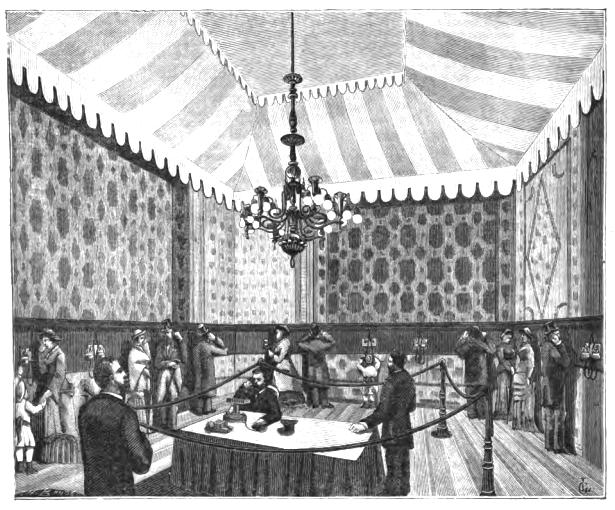
\includegraphics[width=0.99\columnwidth]{CAPITOLI/0300/IMG/1881opr4.jpg}
	\vspace{-10pt}
	\caption[]{Illustrazione della sala d'ascolto del telefono all'Esposizione di
	Parigi del 1881. Gli ascoltatori avevano i ricevitori telefonici per entrambe
	le orecchie per ascoltare il programma teatrale in stereo.}
	\label{fig:teatrophone2}
\end{figure}

Nonostante il telefono fosse un'invenzione giovanissima, al punto da pensare che
la diffusione del suono dal teatro alla sala d'ascolto avrebbe rappresentato
motivo di interesse da parte del pubblico a prescindere dalla condizione di
ascolto, Ader aggiunse l'idea di esperienza che, attraverso i concetti di
binauralità e stereofonia, ebbe un impatto incredibile sul pubblico. L'articolo
comparso su \emph{L'Electricien} in cui si descrive il funzionamento
dell'invenzione fu firmato da M. Hospitaller che descrive così l'esperienza di
ascolto:

\begin{figure}[t]
	\centering
	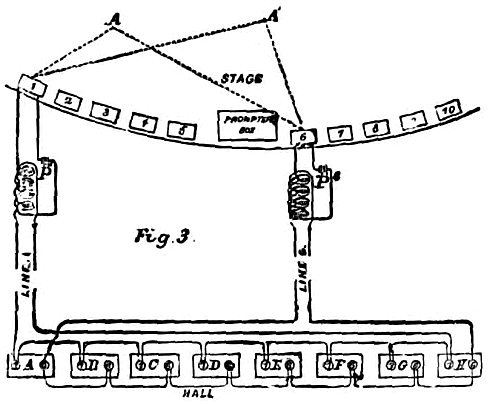
\includegraphics[width=0.99\columnwidth]{CAPITOLI/0300/IMG/1881opr2.jpg}
	\vspace{-10pt}
	\caption[]{Disposizione dei trasduttori sul palco e collegamento alle due linee
	telefoniche. Ogni ascoltatore è posizionata di fronte ad una coppia di telefoni
	i quali ricevono il segnale da due trasduttori distinti posizionati sul palco.
	Questi trasduttori sono raggruppati in coppie forniscono segnale a sedici
	telefoni, accoppiati per otto ascoltatori.}
	\label{fig:teatrophone1}
\end{figure}

\begin{quote}
We will now consider the new acoustic effect which Mr. Ader has discovered, and
applied for the first time in the telephonic transmission at the Electrical
Exhibition. Every one who has been fortunate enough to hear the telephones at
the Palais de l'Industrie has remarked that, in listening with both ears at the
two telephones, the sound takes a special character of relief and localization
which a single receiver cannot produce. [\ldots] As soon as the experiment
commences the singers place themselves, in the mind of the listener, at a fixed
distance, some to the right and others to the left. It is easy to follow their
movements, and to indicate exactly, each time that they change their position,
the imaginary distance at which they appear to be. [\ldots] This phenomenon is
very curious, it approximates to the theory of binauriclar auduition, and has
never been applied, we believe, before to produce this remarkable illusion to
which may almost be given the name of auditive perspective. [\ldots] In order
to realize it, we may recall the stereoscope, which allows us to see objects in
their natural relief\footnote{
\emph{Scientific American}, December 31, 1881, pages 422-423,\\
\url{https://earlyradiohistory.us/1881opr.htm} \\
Considereremo ora il nuovo effetto acustico che il signor Ader ha scoperto e
applicato per la prima volta nella trasmissione telefonica all'esposizione
elettrica. Tutti coloro che hanno avuto la fortuna di ascoltare i telefoni al
\emph{Palais de l'Industrie} hanno osservato che, ascoltando con entrambe le
orecchie ai due telefoni, il suono assume un carattere speciale di meraviglia e
localizzazione, cosa che un singolo ricevitore non può produrre. [\ldots] Non
appena inizia l'esperimento, i cantanti si posizionano, nella mente
dell'ascoltatore, a una distanza fissa, alcuni a destra e altri a sinistra. È
facile seguire i loro movimenti e indicare esattamente, ogni volta che cambiano
posizione, la distanza immaginaria alla quale sembrano essere. [\ldots] Questo
fenomeno è molto curioso, si avvicina alla teoria dell'audizione biauricolare che
crediamo non sia mai stato applicato prima di produrre questa straordinaria
illusione, a cui potrebbe essere dato il nome di prospettiva auditiva. [\ldots]
Per realizzarlo, possiamo ricordare lo stereoscopio, che ci consente di vedere
gli oggetti nel loro rilievo naturale.}.
\end{quote}

Tra le varie definizioni di stereofonia il termine è inoltre usato per indicare
la parte dell’acustica fisiologica che si occupa del fenomeno dell'ascolto
biauricolare del sistema uditivo. Tale fenomeno conferisce alla percezione umana
il potere localizzatore, cioè la capacità, dovuta al lavoro congiunto dei due
sistemi auricolari separati ed al sistema nervoso centrale, di determinare la
direzione di provenienza di un suono. In tal senso, esiste in acustica
fisiologica la definizione di monofonia in qualità di condizione anomala del
sistema percettivo, caratterizzata dalla mancanza degli elementi necessari a
individuare i caratteri spaziali dei suoni stessi, come per esempio quella
ottenuta con un solo orecchio.

La percezione dei caratteri spazio-temporali dei suoni, in particolare della
loro direzione di provenienza e della loro relazione con lo spazio che
attraversano, definiscono i tratti essenziali della stereofonia, in relazione
all'udito, in virtù dell’audizione biauricolare (o binaurale).

\begin{quote}
When recording music considerable trouble is experienced with the unpleasant
effects produced by echoes wich in the normal way would not be noticed by anyone
listening in the room in which the performance is taking place.
An observer in the room is listening with two ears, so that echoes reach him
with the directional significance which he associates with the music performed
in such room. He therefore discount these echoes and psychologically focuses
his attention on the source of the sound. When the music is reproduced through
a single channel the echoes arrive from the same direction as the direct sound
so that confusion results. [\ldots] Human ability to determine the direction
from which sound arrives is due to binaural hearing, the brain being able to
detect differences between sound received by the two ears from the same source
and thus to determine angular directions from which various sounds
arrive\footnote{[\cite{ab58}] - Quando si registra musica acustica, si riscontrano
notevoli problemi a causa degli effetti indesiderati prodotti dalle riflessioni
acustiche dell'ambiente, che nell'ascolto normale non vengono notati dagli
ascoltatori nella stanza in cui si svolge l'esibizione.
Un osservatore nella stanza sta ascoltando con due orecchie, in
modo che gli echi lo raggiungano con il significato direzionale che associa alla
musica eseguita in quella stanza. Pertanto, non tiene conto di questi echi e
focalizza psicologicamente la sua attenzione sulla fonte del suono. Quando la
musica viene riprodotta attraverso un singolo canale, gli echi arrivano dalla
stessa direzione del suono diretto, in modo da creare confusione. [...] La
capacità umana di determinare la direzione da cui proviene il suono è dovuta
all'udito binaurale, il cervello è in grado di rilevare le differenze tra il
suono ricevuto dalle due orecchie dalla stessa fonte e quindi di determinare le
direzioni angolari da cui provengono i vari suoni.}.
\end{quote}

È con queste parole che \adb~ nel 1931 descriveva i fondamenti delle conoscenze
in termini di percezione dei suoni e di come questi venivano utilizzati per definire
criteri tecnologici adeguati per la riproduzione dei suni. Ed è per questo che
in maniera piuttosto discreta intitola testo del brevetto che ha dato la nascita
commerciale e tecnologica alla stereofonia \emph{Miglioramenti in, ed in relazione,
ai sistemi di trasmissione del suono, registrazione del suono e riproduzione del suono}.
Genrico, inglese, la binauralità dell'ascolto umano è la prima affermazione di
Blumlein: “\emph{un osservatore nella stanza sta ascoltando con due orecchie}”.
Come questa condizione di ascolto si evolva nel tempo è la peculiarità della
stereofonia.

Il documento presenta diverse tecniche stereofoniche di microfonazione, di
incisione del disco e di trasmissione radio. La domanda fu presentata nel
dicembre 1931 ed approvata nel giugno 1933. Nel testo fa riferimento al cinema,
consapevole della necessità di migliorare la resa della registrazione sonora
in situazioni di “realismo”.

\emph{Una voce in una piccola stanza riverberante è una condizione d'ascolto che
rispetti qualità di stereofonia?}

In funzione di dei riferimenti storici e delle descrizioni fatte finora, la
risposta è chiaramente affermativa. Anche con un solo oggetto sonoro, una sola
voce, in una piccola stanza, siamo in presenza di un fenomeno acustico
stereofonico, percepito bianuralmente. Su questa condizione Blumlein presenta
le basi teoriche e tecnologiche della stereofonia, nel brevetto in cui ne
rende i concetti fondamentali, solidi, stabili nel tempo e nello spazio delle parole.

\vfill\null

\begin{figure}[bh]
\begin{bio}[Alan Dower Blumlein]
	Nato il 29 giugno 1903 a Londra, Deceduto il 7 giugno 1942 a Herefordshire,
	Inghilterra, fu ingegnere elettronico presso EMI, per la quale pubblicò brevetti
	per le sue numerose invenzioni nel campo delle telecomunicazioni soprattutto in
	relazione alle tecnologie di registrazione, trasmissione e diffusione del suono.
	Ottiene, nella sua breve carriera, 128 brevetti, motivo per cui è considerato
	uno dei più importanti ingegneri e inventori del suo tempo. Morì durante la
	seconda guerra mondiale all'età di 38 anni, durante un test militare segreto del
	sistema radar H2S allora in fase di sviluppo, a bordo del bombardiere Halifax
	su cui stava volando. Tra le numerose invenzioni legate al nome di Blumlein
	quelle legate alla Stereofonia stravolsero completamente il mondo della
	fruizione pubblica del suono. Le sue prime note sull'argomento risalgono al 25
	settembre 1931 e il suo brevetto aveva il titolo “Miglioramenti ai, ed in
	relazione ai, sistemi di trasmissione, registrazione e riproduzione del suono”.
	La domanda di brevetto fu del 14 dicembre 1931 ed la concessione fu dell
	14 giugno 1933, brevetto britannico numero 394.325.
\end{bio}
\end{figure}

% \vfill\null
%
% %------------------------- APPROFONDIMENTO
% %\begin{figure}[th]
% \begin{table}[ht]
% \footnotesize
% \begin{tabular}{L{.969\textwidth}}%
% \toprule
% 	\textbf{Michael Antony Gerzon}\\
% \midrule
% Nato il 4 dicembre 1945, deceduto il 6 maggio 1996. Matematico, all'università
% aveva già un forte interesse sia per la teoria che per la pratica della
% registrazione, che condivideva con alcuni colleghi studenti tra cui Peter Craven
% (i due furono in seguito i co-inventori del microfono \emph{Soundfield} e
% collaborarono a molti altri progetti). Dagli nei primi anni settanta sviluppa la
% tecnologia \emph{Ambisonics}, che può essere descritta come un completamento teorico
% e pratico del lavoro svolto da Alan Blumlein nel campo del suono stereofonico.
% Gerzon morì nel 1996 per complicazioni dovute a un grave attacco d'asma. \\
% \bottomrule
% \end{tabular}
% \end{table}
% %\end{figure}
% %------------------------- APPROFONDIMENTO


%%%%%%%%%%%%%%%%%%%%%%%%%%%%%%%%%%%%%%%%%%%%%%%%%%%%%%%%%%%%%%%%%%% SECTION FOUR
%%%%%%%%%%%%%%%%%%%%%%%%%%%%%%%%%%%%%%%%%%%%%%%%%%%%%%%%%%%%%%%%%%%%%%%%%%%%%%%%
\section{Ramificazioni}

Abbiamo chiarito, con l'ausilio delle parole di Blumlein, che una voce in
una piccola stanza riverberante è una condizione d'ascolto stereofonica.

\begin{quote}
When recording music considerable trouble is experienced with the unpleasant
effects produced by echoes wich in the normal way would not be noticed by anyone
listening in the room in which the performance is taking place. [\ldots]
When the music is reproduced through a single channel the echoes arrive from
the same direction as the direct sound so that confusion results.
\end{quote}

Con la profonda conoscenza del significato del tempo trascorso tra noi e Blumlein,
si può ora esporre il significato dello strumento altoparlante in maniera più
dettagliata e consapevole. Per l'era Blumlein, l'altoparlante era lo strumento
futuro per un tempo presente migliore. Il suono riprodotto, alla sua giovane età,
era pura magia. Oggi sappiamo bene quanto siamo insoddisfatti della riproduzione
dei suoni acustici attraverso agli altoparlanti. Quando il primo \emph{iPhone} è
stata l'unica cosa intelligente sul pianeta è stato fantastico, un fantastico
oggetto di creazione. Oggi con lo stesso oggetto non faremmo nemmeno una foto.
Ascoltare un assolo di violino riprodotto dal miglior altoparlante sul mercato
non rappresenta la stessa esperienza della performance reale. L'insoddisfazione
dell'artificio non è legata solo ai principi di stereofonia o all'abilità tecnica
con cui l'artificio viene prodotto, essa è parte integrante del limite intrinseco
nella tecnologia di riproduzione che siamo in grado di realizzare.

Sostituendo la voce umana con la sua registrazione riprodotta da un singolo
altoparlante perdiamo, come descritto da Blumlein, la capacità del sistema
orecchie-cervello di decifrare la relazione originaria tra sorgente sonora, suono
come movimento e ambiente. Non è più lo stesso ascolto stereofonico. Diventa un
altro ascolto, una nuova condizione di ascolto. Il numero di fonti è lo stesso.
Entrambi nel loro linguaggio monofonico producono una diversa condizione di ascolto.

Nel 1992 \mg, in uno dei suoi molti tentativi di descrivere
metodologie di ascolto stereofonico, disegna una rappresentazione schematica
delle diverse posizioni che possono assumere gli altoparlanti in
configurazioni stereo, con configurazioni da uno a cinque diffusori:

\begin{quote}
\ldots we show the loudspeaker layouts considered for frontal stage stereo
using from one (regarding mono as the trivial case of “one-loudspeaker stereo”!)
to five loudspeakers\footnote{\cite{mg:92pdmsss} - mostriamo le disposizioni
degli altoparlanti considerati per lo stereo frontale partendo da uno
(considerando il mono come il banale caso dello “stereo con un solo altoparlante”!}.
\end{quote}

\emph{Esiste una condizione di stereofonia possibile con un solo altoparlante?}
Ovviamente si, ma non è nella riproduzione del violino che la percepiamo.

Ci si trova in quella magica condizione di ascolto stereofonico da un solo
altoparlante quando questo è messo in condizione di suonare se stesso, il suo
mondo elettrico, svincolato dalla riproduzione di qualcosa di acustico. Un
altoparlante solo può essere messo nella condizione stereofonica di produrre un
suono che non esisterebbe altrimenti, con caratteristiche e risultati
psico-acustici generali di stereofonia e percezione binaurali assimilabili alla
voce parlante dell'esempio di Blumlein.
Un rumore rosa filtrato in una banda molto stretta e mobile attorno al punto di
taglio di un crossover interno ad un diffusore a due vie che canta
monofonicamente in una stanza, è una meravigliosa condizione di stereofonia
attraverso un canto monofonico. Ripreso con una tecnica stereofonica avrebbe la
stessa dignità stereofonica del suono di un violino.

%\subsection{Sullo strumento \emph{Altoparlante}}

L'enciclopedia britannica cataloga con una inequivocabile descrizione il termine
\emph{loudspeaker: sound instrument}. Il passaggio da altoparlante come strumento
sonoro ad altoparlante come strumento musicale è breve: è necessario solo
aggiungere il musicista.

La scelta dell'altoparlante, la conoscenza del suo carattere e delle caratteristiche
tecniche è un momento necessario per quel musicista, un momento che richiede tempo.
Cambiare manualmente la frequenza di un suono sinusoidale riprodotto da un diffusore è un
buon modo per conoscere l'altoparlante. Il musicista scoprirà in questo modo che i
suoni prodotti dall'altoparlante cambieranno forma durante il glissato. Forse
troverà alcune peculiarità, o strane caratteristiche che richiederanno ulteriore
studio. L'ambiente stesso si troverà in condizioni mutevoli di relazione con il suono riprodotto.

Scoprire e conoscere lo strumento altoparlante e conoscere il sistema percettivo
in termini di meccanismi psico-acustici sono condizioni necessarie per
affrontare correttamente un percorso di emancipazione nei confronti dei limiti
tecnici e tecnologici nella riproduzione e nella produzione elettroacustica dei suoni.

%%%%%%%%%%%%%%%%%%%%%%%%%%%%%%%%%%%%%%%%%%%%%%%%%%%%%%%%%%%%%%%%%%%% SUBSECTION
%%%%%%%%%%%%%%%%%%%%%%%%%%%%%%%%%%%%%%%%%%%%%%%%%%%%%%%%%%%%%%%%%%%%%%%%%%%%%%%%
\subsection{Spazio, spazializzazione e \emph{PanPot}}
\label{sec:panpot}

L'uso di parole inappropriate negli ambiti delle tecniche e tecnologie audio ha prodotto
alcuni sistemi di riferimento a loro volta inadeguati. Il sistema di diffusione
stereofonico \emph{left-right} si è imposto discograficamente e nell'industria
delle telecomunicazioni ed ha generato la convinzione che il numero due
rappresenti l'optimum per la difusione stereofonica e non il minimum.
A questo ci si può aggiungere che attualmente non si ha la minima propensione
all'ascolto acustico. A causa di queste inappropriate condizioni culturali
ci si trova quotidianamente a confondere concetti di stereofonia,
spazializzazione, movimento del suono e proiezione sonora. Ognuno di questi
argomenti cruciali per le materie elettroacustiche verranno discussi con i
dovuti approfondimenti. Nonostante ciò prima di entrare nel pieno della sterofonia
pratica va descritta almeno la condizione minima del sistema \emph{left-right}.

L'oggetto \emph{panner} è rappresentato da un potenziometro di controllo
(hardware o software, in entrambi i casi a controllo analogico o digitale) che
regola la distribuzione di un segnale su più canali componenti un campo sonoro
stereo o multicanale. Ogni mixer ha un \emph{panpot} (abbreviazione di
\emph{potenziometro di panoramica}), per ciascun canale sorgente in ingresso,
che regola l'azione del \emph{panner}. Generalmente il \emph{panpot} viene descritto come un pomello che permette di
muovere i suoni tra la sinistra e la destra del panorama di diffusione, il che è
parzialmente vero e potenzialmente pericoloso in termini di immaginazione
acustica. Soffermandosi ad analizzare il fenomeno acustico di un suono prodotto da un
oggetto in movimento tra la destra e la sinistra di un campo percettivo emergono
diversi problemi. Il primo riguarda l'\emph{effetto doppler}.

\begin{figure*}[t!]
    \centering
    \begin{subfigure}[t]{0.45\textwidth}
        \centering
        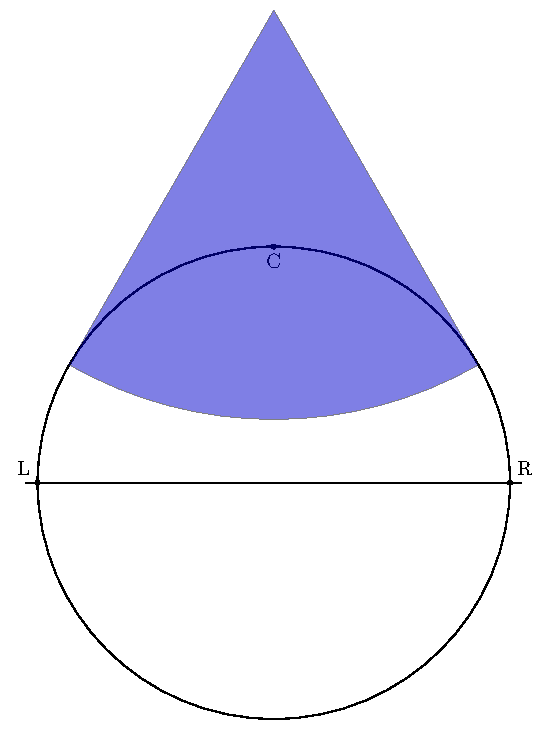
\includegraphics[height=8cm]{CAPITOLI/_TIKZ/PANNING/pan-frontal}
        \caption[]{Sorgente con incidenza frontale.}
        \label{pan:frontal}
    \end{subfigure}%
    ~
    \begin{subfigure}[t]{0.45\textwidth}
        \centering
        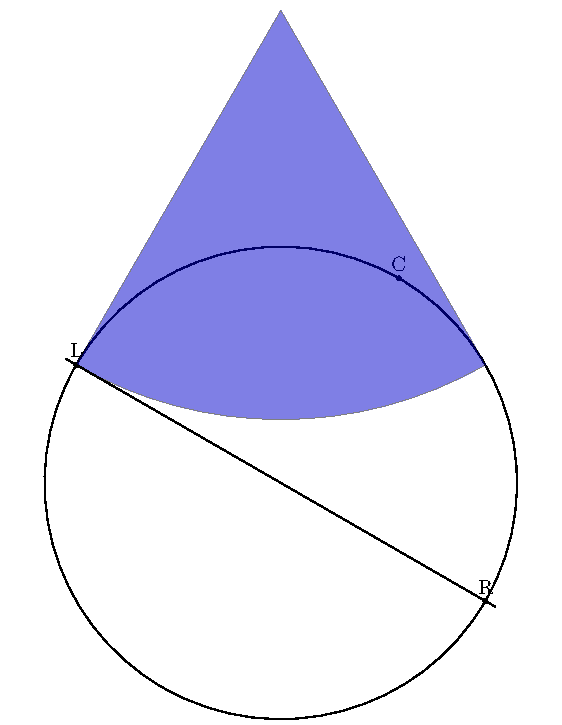
\includegraphics[height=8cm]{CAPITOLI/_TIKZ/PANNING/pan-left}
        \caption[]{Sorgente con incidenza laterale sinistra di 30 gradi.}
        \label{pan:left}
    \end{subfigure}
    \\
    \begin{subfigure}[t]{0.9\textwidth}
        \centering
        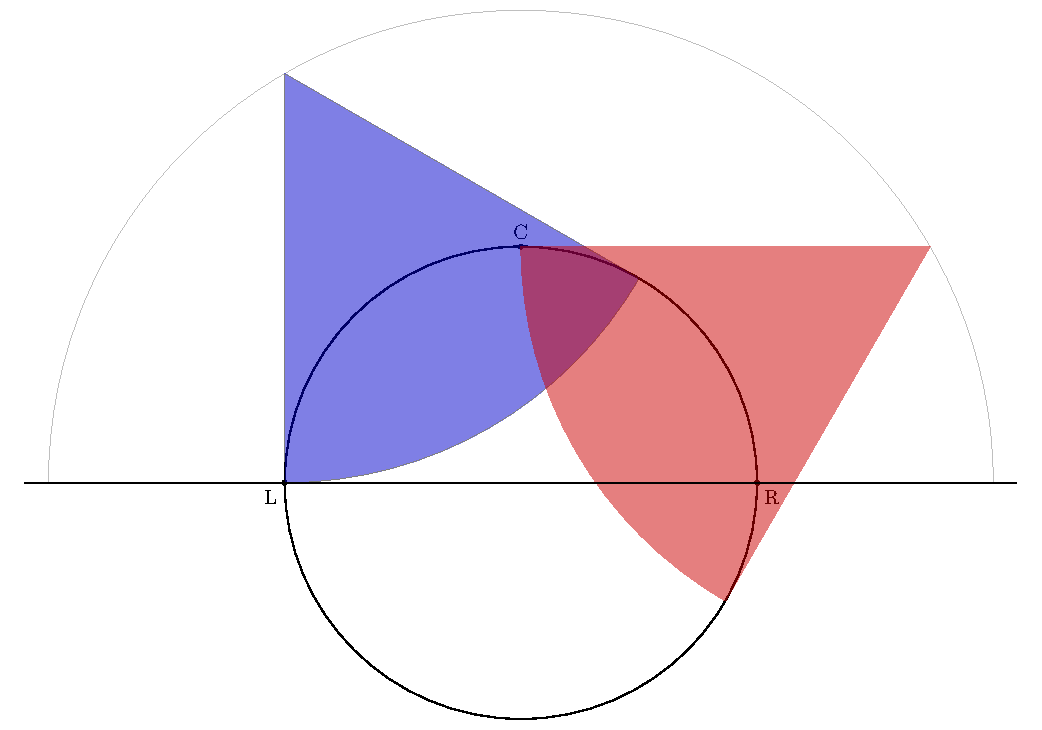
\includegraphics[height=8cm]{CAPITOLI/_TIKZ/PANNING/pan-both}
        \caption[]{Due sorgenti, una con incidenza laterale sinistra di 30 gradi,
        l'altra con incidenza laterale destra di 60 gradi.}
        \label{pan:both}
    \end{subfigure}
    \caption[]{La rotazione del \emph{PanPot} esegue una modifica della condizione
    di ascolto dell'ascoltatore, non un movimento della sorgente. Posizionando
    le singole sorgenti ci si pone in ascolto laterale, ruotati. Nella
    sovrapposizione di molteplici sorgenti il panorama risulta composto da
    ognuna di queste, con posizioni assolute ed angoli di incidenza relativi
    della testa.}
    \label{pan:all}
\end{figure*}

Siamo seduti su una panchina al
margine di una strada che si estende infinita agli estremi della nostra vista
periferica. Un mezzo di soccorso, con la sirena accesa, si avvicina percorrendo
la strada davanti al nostro viso, da sinistra verso destra: percepiamo
una variazione in frequenza al passaggio della sirena, in funzione della
velocità. L'\emph{effetto doppler} ci descrive come nel percorso di
avvicinamento a noi la frequenza sale lentamente fino al massimo ottenuto nel
momento in cui ci raggiunge per poi diminuire rapidamente in coincidenza con
l'allontanamento. Ora siamo dei \emph{sound designer}, siamo seduti di fronte alla nostra console
analogica e dobbiamo replicare l'effetto sopra descritto. Applicando un
movimento da sinistra a destra, azionando il \emph{panpot} su un suono di sirena
statico, registrato fermo ad un metro di distanza, pur ruotando velocemente il
potenziometro non otteniamo variazioni in frequenza. Il suono si muove tra la
sinistra e la destra del sistema d'ascolto senza produrre il movimento nello
spazio ma solamente lo spostamento della posizione relativa al nostro punto di
ascolto. Ne deriva una prima conslusione: il \emph{panpot} regola una posizione
relativa, non stabilisce criteri di movimento. Un altro problema emergente del
pensare il \emph{panning} come un movimento
scaturisce dalla relazione della sorgente con l'ambiente circostante. Che
movimento può esserci senza tenere conto del luogo in cui la sorgente sonora si
trova?

\begin{figure}[t!]
\centering
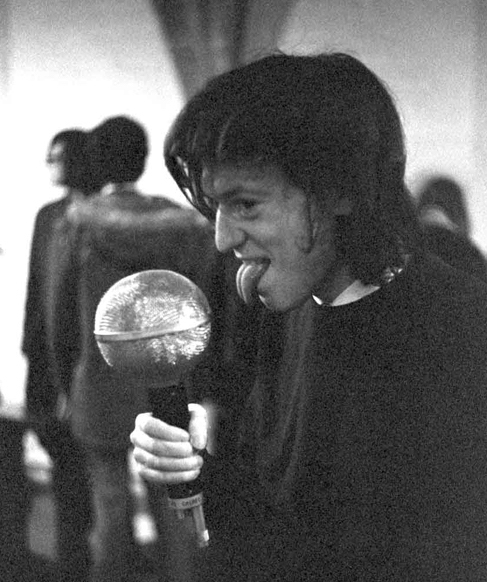
\includegraphics[width=0.99\columnwidth]{CAPITOLI/0300/IMG/MAG-licking-G-web.jpg}
\caption[]{Michael Gerzon}
\label{ph:mg1}
\end{figure}

Un avvocato pronuncia la sua arringa in tribunale parlando ad alta voce,
camminando, rimbalzando tra destra e sinistra. La voce si propaga nello spazio
ed è inevitabile che se ne percepisca la variazione topologica, morfologica in
relazione con le caratteristiche architettoniche: a sinistra della stanza c'è
una parete di finestre, a destra un muro in cemento. Pur non avendo velocità
sufficiente ad innescare l'effetto doppler, la sua continua variazione di
posizione corrisponde ad una continua variazione di rapporto con l'ambiente che
lo circonda, in relazione ad ogni infinto punto di ascolto all'interno della
stanza. In altre parole, quel movimento assume significati diversi relativi al
punto di ascolto. Dovendo simulare lo stesso effetto mediante l'azione sul panpot, otterremmo la
variazione di posizione della voce nello spazio, ma non la sua relazione con lo
spazio.

Il \emph{panpot}, nella sua capacità di descrizione della relazione tra i canali
che ricevono i suoi segnali, non muove la sorgente nello spazio, ma regola la
posizione della sorgente stessa in relazione al nostro punto di ascolto. In
altri termini il \emph{panner} non regola il movimento della sorgente, ma la
rotazione della testa in relazione ad essa. Il \emph{panner}, muove langolo di
incidenza del suono, ruota la testa, nei confronti della sorgente immobile.

Ogni \emph{panner} ha un'architettura interna che determina la quantità e la
condizione del segnale sorgente per ogni canale di destinazione. I più semplici
suddividono i segnali audio nei due canali sinistro e destro, attraverso un
opportuno controllo di guadagno (volume) discreto. La distribuzione dell'energia
tra i due canali è chiamata legge ed è descrivibile con una funzione matematica.

Come descritto da Blumlein, la sola variazione di ampiezza nella
rappresentazione del panorama stereofonico rappresenta una parte nella complessa
soddisfazione della percezione binaurale, non disegna l'intero meccanismo.
Per questo motivo, prima di descrivere i sistemi di panning di ampiezza, che
sono universalmente implementati su tutti i mixer del pianeta, è più opportuno
riprendere da dove egli stesso è partito. La visione di Blumlein fu ripresa in
seguito da Michael Gerzon, negli anni settanta, per sviluppare la tecnologia
\emph{ambisonic}, la quale rimane un atto di descrizione del mondo sonoro
percepito e riprodotto, nell'evoluzione del concetto di stereofonia, completamente diverso
da quello che commercialmente si è diffuso ed imposto, per il semplice tentativo
di colmare il divario con il regno acustico.

\begin{quote}
The ears and brain localize sounds according to many different mechanisms. Among
the most important cues used are low-frequency interaural phase (applicable up
to around $2KHz$, but dominant below $700Hz$) and localization by
amplitude differences between the two ears, predominantly above about
$1KHz$. While other cues are also important, we have found that satisfying
both these cues, and making them mutually consistent for central listener facing
in any direction, leads to particularly robust and reliable localization
quality.\footnote{\cite{mg92pdmsss} - Le orecchie e il cervello localizzano i
suoni secondo molti meccanismi diversi. Tra i segnali più importanti utilizzati
vi sono la fase interaurale a bassa frequenza (applicabile fino a circa $2KHz$,
ma dominante al di sotto di $700Hz$) e la localizzazione mediante
differenze di ampiezza tra le due orecchie, prevalentemente al di sopra di
circa $1KHz$. Sebbene anche altri segnali siano importanti, abbiamo
scoperto che soddisfare entrambi questi segnali e renderli reciprocamente
coerenti per l'ascoltatore centrale rivolto verso qualsiasi direzione, porta
a una qualità di localizzazione particolarmente solida e affidabile.}
\end{quote}

\vfill\null

\begin{figure}[bh]
\begin{bio}[Michael Antony Gerzon]
  Nato il 4 dicembre 1945, deceduto il 6 maggio 1996. Matematico, all'università
  aveva già un forte interesse sia per la teoria che per la pratica della
  registrazione, che condivideva con alcuni colleghi studenti tra cui Peter Craven
  (i due furono in seguito i co-inventori del microfono \emph{Soundfield} e
  collaborarono a molti altri progetti). Dagli nei primi anni settanta sviluppa la
  tecnologia \emph{Ambisonics}, che può essere descritta come un completamento teorico
  e pratico del lavoro svolto da Alan Blumlein nel campo del suono stereofonico.
  Gerzon morì nel 1996 per complicazioni dovute a un grave attacco d'asma.
\end{bio}
\end{figure}


% %%%%%%%%%%%%%%%%%%%%%%%%%%%%%%%%%%%%%%%%%%%%%%%%%%%%%%%%%%%%%%%%% SECTION FIVE
% %%%%%%%%%%%%%%%%%%%%%%%%%%%%%%%%%%%%%%%%%%%%%%%%%%%%%%%%%%%%%%%%%%%%%%%%%%%%%%
\section{Mid-Side}

Harvey Fletcher, fisico americano, nel 1934 firma uno degli articoli che
compongono un testo cardine per la storia della tecnologia sonora
“\emph{Symposium on Auditory Perspective}”, sulla percezione e la trasmissione
della musica dal vivo, che inizia con le seguenti parole:

\begin{quote}
In this electrical era one is not surprised to hear that orchestral music can be
picked up in one city, transmitted a long distance, and reproduced in another.
Indeed, most people think such things are commonplace. They are heard every
night on the radio. However, anyone who appreciates good music would not admit
that listening even to the best radio gives the emotional thrill experienced in
the concert hall. \cite{hf34}
\end{quote}

Oggi abbiamo perso ogni scintilla di “quell'era elettrica”, anche quella che ha
suscitato la fiamma di interesse nell'ascolto della musica orchestrale
attraverso la trasmissione.

%, o quella che ha suscitato la fiamma di interesse
% nell'ascolto della musica orchestrale, o quella dell'interesse nell'ascolto o,
% molto più semplicemente, la fiamma dell'di interesse. Cento anni dopo quella
% “era” siamo scimmie. Dobbiamo considerare questo fallimento. Inadempienza. Dobbiamo considerare che
% un libro, anche il più inadeguato, in quanto oggetto di pensiero ha potere, come
% dimostrato nell'introduzione, che potrebbe essere il potere di distruggere.

Nel 1964, Paul W. Klipsch introdusse la ristampa del “\emph{Symposium}”:

\begin{quote}
The following paper is a reprint of one of the most important papers in the
field of audio. Fundamentals do not change. The laws of physics endure. In
reprinting the Symposium, the fundamentals are restated. \cite{sap1964}
\end{quote}

Il testo di Fletcher \cite{hf34} è datato 1934, un anno dopo l'approvazione
del brevetto Blumlein che descrive il concetto fondamentale di trasmissione e
registrazione del suono \emph{Mid-Side}. In quell'epoca gli interessi commerciali e
quelli di ascolto erano intrecciati, in una forma \emph{stereo} solida.

Parlando di orecchie e attività cerebrali per determinare la direzione di una
fonte Blumlein ha scritto:

\begin{quote}
…it is fairly well established that the main factor having effect are phase
differences and intensity differences between the sounds reaching the two ears,
the influence with each of these has depending upon the frequency of the sounds
emitted. For low frequency sound waves there is little or non difference in
intensity at the two ears but there is a marked phase difference. For a give
obliquity of sound the phase difference is approximately proportional to
frequency, representing a fixed time delay between sound arriving at the two
ears, by noting which there is a phase difference of $\pi$ radians or more
between sound arriving at the two ears from a source located on the line joining
them: but above such frequency if phase difference were the sole feature relied
upon for directional location there would be ambiguity in the apparent position
of the source. At the stage however the head begins to became effective as a
baffle and causes noticeable intensity difference between the sounds reaching
the two ears, and it is by noting such intensity difference that brain
determines direction of sounds at higher frequencies\footnote{\cite{ab58} - ...è abbastanza
accertato che il fattore principale sia dovuto alle differenze di fase e di
intensità tra i suoni che raggiungono le due orecchie, l'influenza con ognuna di
queste differenze ha a seconda della frequenza dei suoni emessi. Per le onde
sonore a bassa frequenza c'è poca o nessuna differenza di intensità alle due
orecchie ma c'è una marcata differenza di fase. Per dare un'obliquità del suono,
la differenza di fase è approssimativamente proporzionale alla frequenza, che
rappresenta un ritardo fisso tra il suono che arriva alle due orecchie, notando
che c'è una differenza di fase di $\pi$ radianti o più tra il suono che arriva
alle due orecchie da una sorgente situata sulla linea che le unisce: ma al di
sopra di tale frequenza se la differenza di fase fosse l'unica caratteristica
su cui si basava per la posizione direzionale, ci sarebbe ambiguità nella
posizione apparente della sorgente. Tuttavia, nella fase in cui la testa inizia
a diventare efficace come un deflettore e causa una notevole differenza di
intensità tra i suoni che raggiungono le due orecchie, ed è notando tale
differenza di intensità che il cervello determina la direzione dei suoni a
frequenze più alte.}.
\end{quote}

Sulla base della conoscenza dei meccanismi sopra esposti Blumlein ha formulato
la maggior parte dei principi fondamentali impressi nella storia della stereofonia.
L'approccio più semplice descritto permette di ottenere semplici differenze di
livello nella riproduzione dagli altoparlanti, percepite come differenze di
livello e di fase dalle orecchie. Per ottenere questo tipo di segnale sono
necessari almeno due microfoni posizionati tra loro vicinissimi, allineati
verticalmente, in modo da non avere alcun ritardo (orizzontale) tra i canali.
Questa configurazione definita \emph{coincidente} è l'ideale per alimentare
gli altoparlanti con differenze pure di ampiezza tra i canali. Una delle tipiche
tecniche di ripresa stereofonica per coppia coincidente prende proprio il nome
da Blumlein: due microfoni bidirezionali, figura-8 quindi a gradiente di pressione,
angolati tra loro di $\pm45$ gradi, in modo da avere un angolo retto tra loro.

Tuttavia, come esposto nel brevetto, i soli microfoni disponibili a Blumlein nei
suoi primi esperimenti erano dinamici non-direzionali a pressione. Coppie
stereofoniche coincidenti con microfoni di questo tipo non sono possibili, in
quanto il loro allineamento verticale produrrebbe due segnali identici, che non
descriverebbero stereofonia. È necessaria quindi una distanza tra i due microfoni.
Due microfoni non-direzionali distanziati anche poco tra loro sono in grado di
produrre segnali quasi identici in ampiezza ma diversi in fase. Blumlein quindi
si concentra su una strategia per produrre anche una differenza di ampiezza tra
i due microfoni, inserendo un blocco di legno tra i due microfoni e progettando
una matrice elettrica che mettesse in relazione i due segnali in modo da
produrre le giuste differenze di ampiezza nell'altoparlante. Il prodotto di tale
ricerca fu la matrice di somma e differenza alla base della tecnologia
\emph{Mid-Side}.

\begin{quote}
\ldots a system of sound transmission wherein the sound
is receive by two or more microphones, wherein at low frequencies difference in
the phase of sound pressure at the microphone is reproduced as difference in
volume at the loud speaker. [\ldots] two microphones transmitted over individual
channels are adapted to interact [\ldots] consisting in half of the sum and half
of the difference respectively of the original \cite{ab58}
\end{quote}

\begin{figure*}[b!]
    \centering
    \begin{subfigure}[t]{0.48\textwidth}
        \centering
        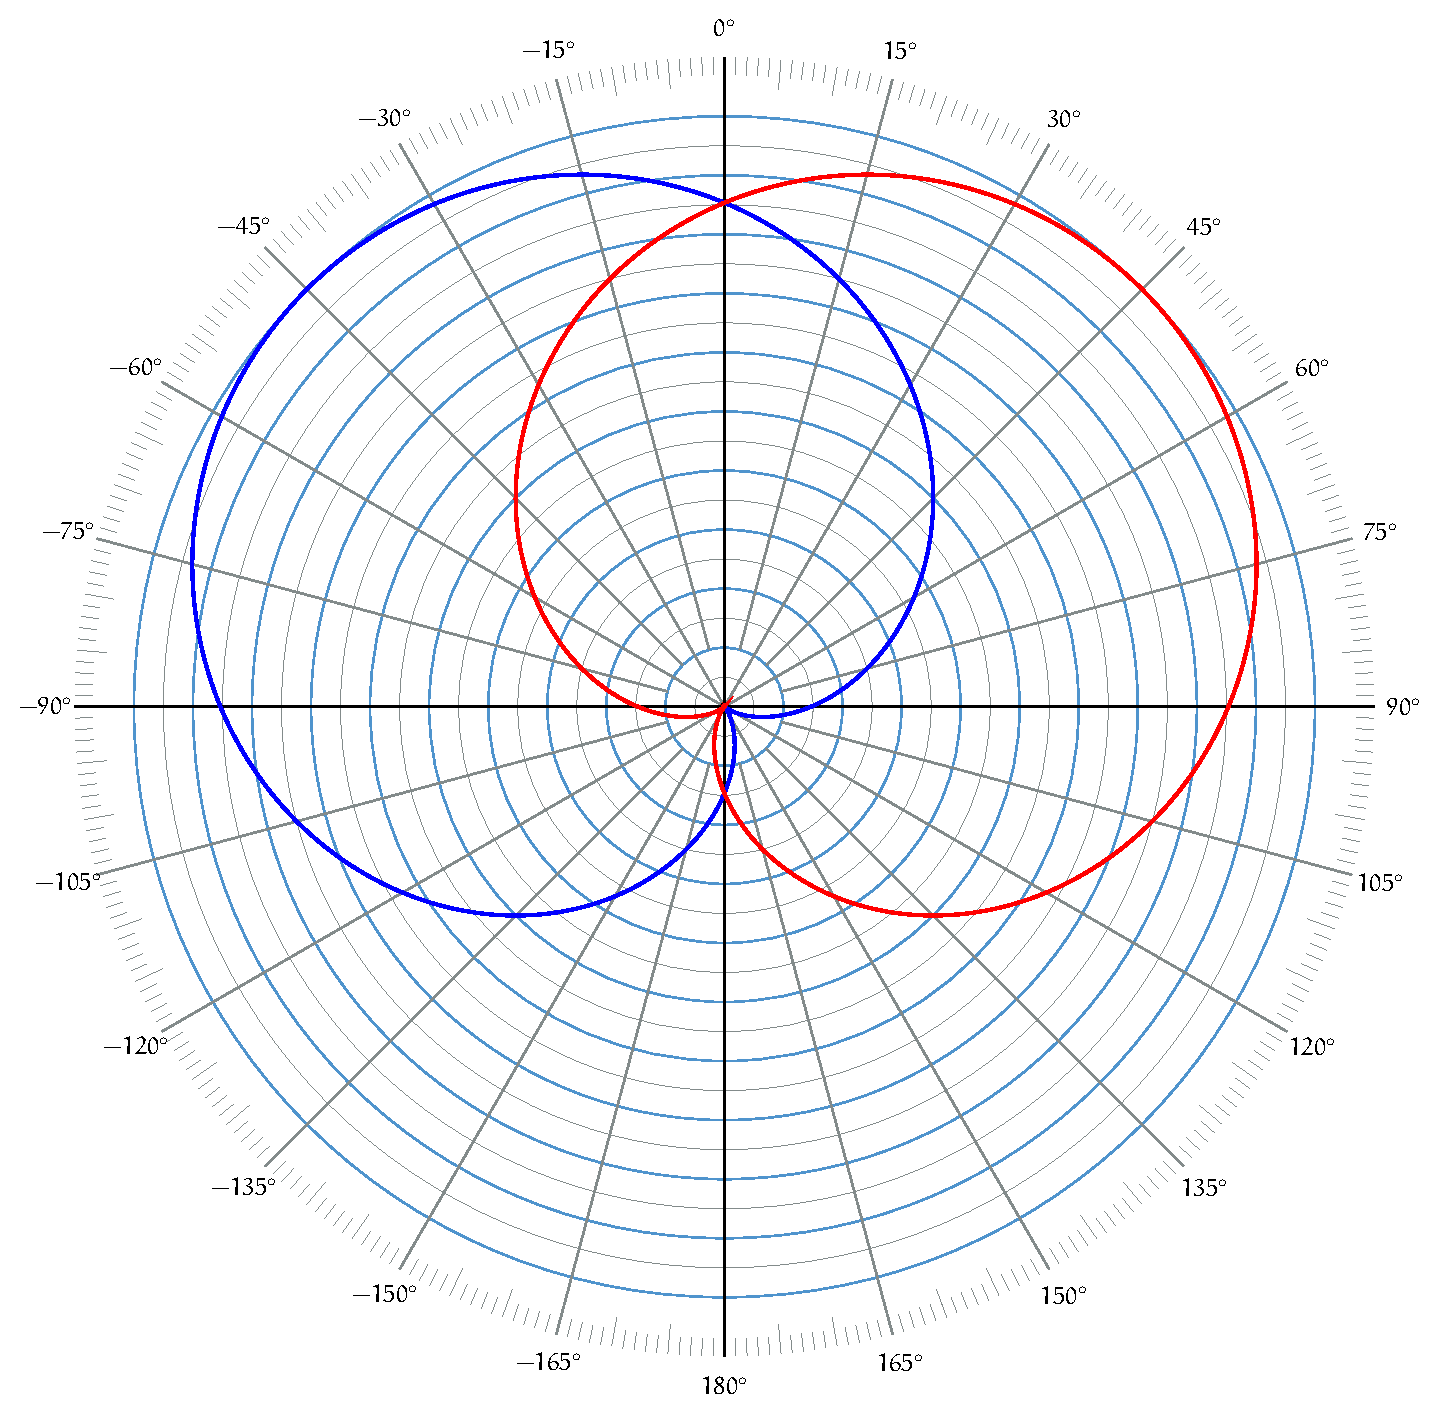
\includegraphics[height=6cm]{microphone-polar-patterns/xy90}
        \caption[]{Coppia stereofonica coincidente di cardioidi angolati di 90 gradi tra loro in entrata alla matrice.}% \\ Eq: $1(x)$}
        \label{pol:xy90ms}
    \end{subfigure}%
    ~
    \begin{subfigure}[t]{0.48\textwidth}
        \centering
        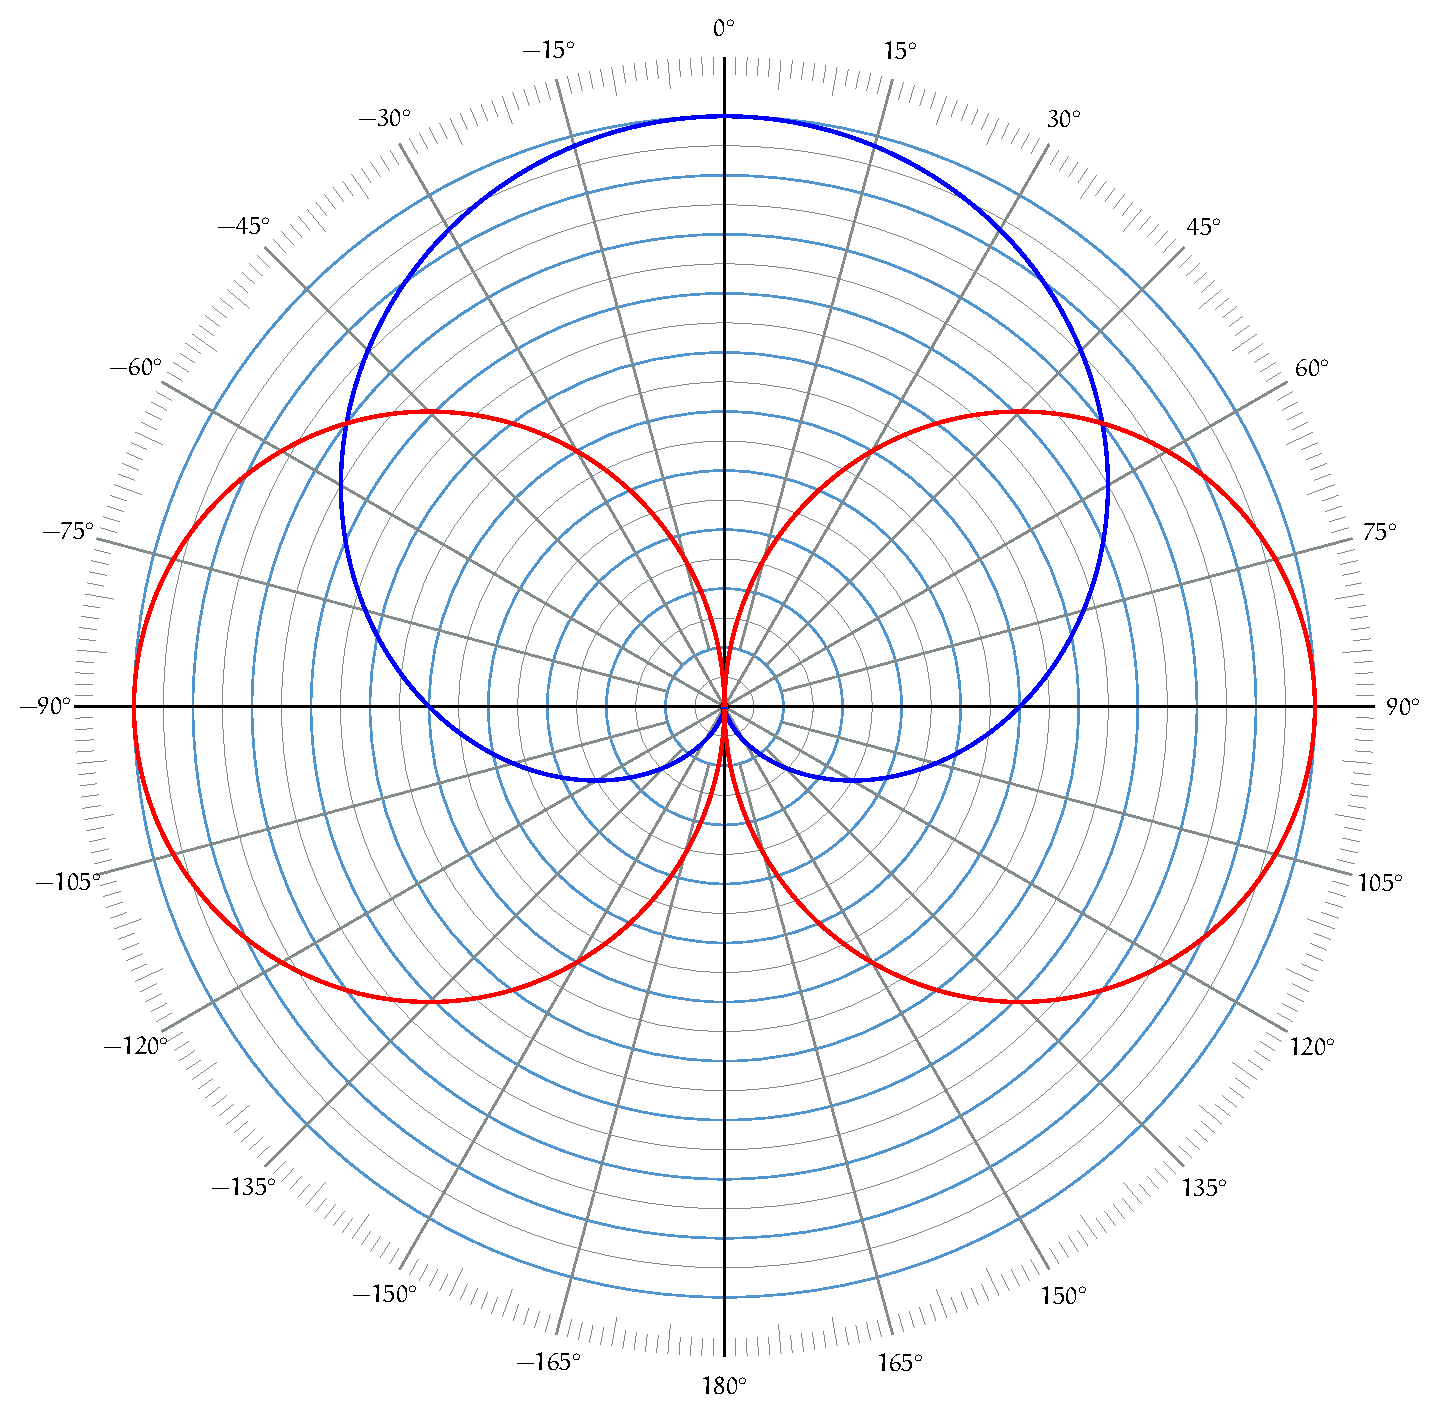
\includegraphics[height=6cm]{microphone-polar-patterns/midside}
        \caption[]{Le componenti \emph{Mid-Side} in uscita.}% \\ Eq: $0.75(x)+0.25(x\cos\theta)$}
        \label{pol:midsidems}
    \end{subfigure}
    \caption[]{Rappresentazione polare ideale del transito di una coppia \emph{xy90}
    attraverso la matrice e relativa rappresentazione d'uscita \emph{Mid-Side}.}
    \label{pol:msmatrix}
\end{figure*}

La matrice di Blumlein di somma e differenza tra i segnali è bidirezionale.
Quando il canale sinistro e destro di una coppia stereofonica passa attraverso
la matrice, la somma di entrambi i canali fornisce il segnale \emph{Mid}
contenente solo le componenti in fase, mentre la differenza produce il segnale
\emph{Side} laterale contenente solo componenti non in fase tra loro. Quando
sono le componenti \emph{Mid-Side} a transitare attraverso la matrice, la somma
di \emph{Mid} e \emph{Side} fornisce la correlazione tra fase sinistra e ampiezza,
mentre la differenza produce la correlazione tra fase negativa a ampiezza.

Di seguito il codice \emph{Faust} per la matrice somma e differenza.

%--------------------------------------------
%----------------larghezza massima del codice
\begin{lstlisting}
nsum = 0.5*(_+_);
ndif = 0.5*(_-_);
sdmx = _,_ <: nsum, ndif;
\end{lstlisting}

\begin{figure}[ht]
  \centering
  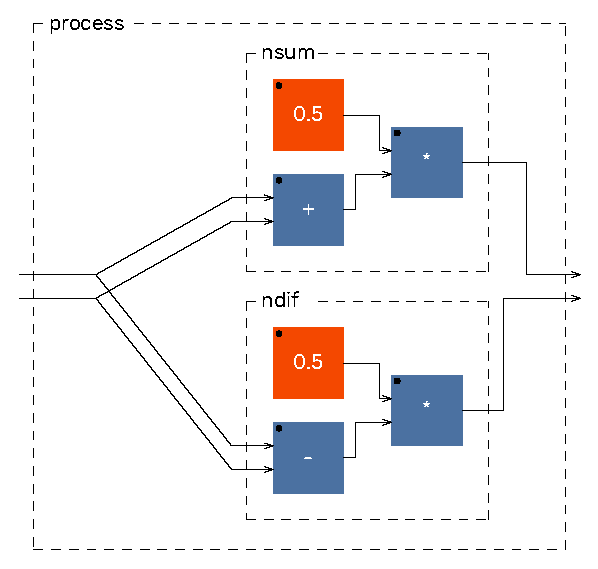
\includegraphics[]{CAPITOLI/0300/IMG/sdmx}
  \caption[]{Matrice somma e sottrazione.}
  \label{bd:sdmx}
\end{figure}

%%%%%%%%%%%%%%%%%%%%%%%%%%%%%%%%%%%%%%%%%%%%%%%%%%%%%%%%%%%%%%%%%%%% SECTION SIX
%%%%%%%%%%%%%%%%%%%%%%%%%%%%%%%%%%%%%%%%%%%%%%%%%%%%%%%%%%%%%%%%%%%%%%%%%%%%%%%%
\subsection{Mid-Side \emph{mic}}
\label{subsec:msmic}

\begin{figure}[b!]
\centering
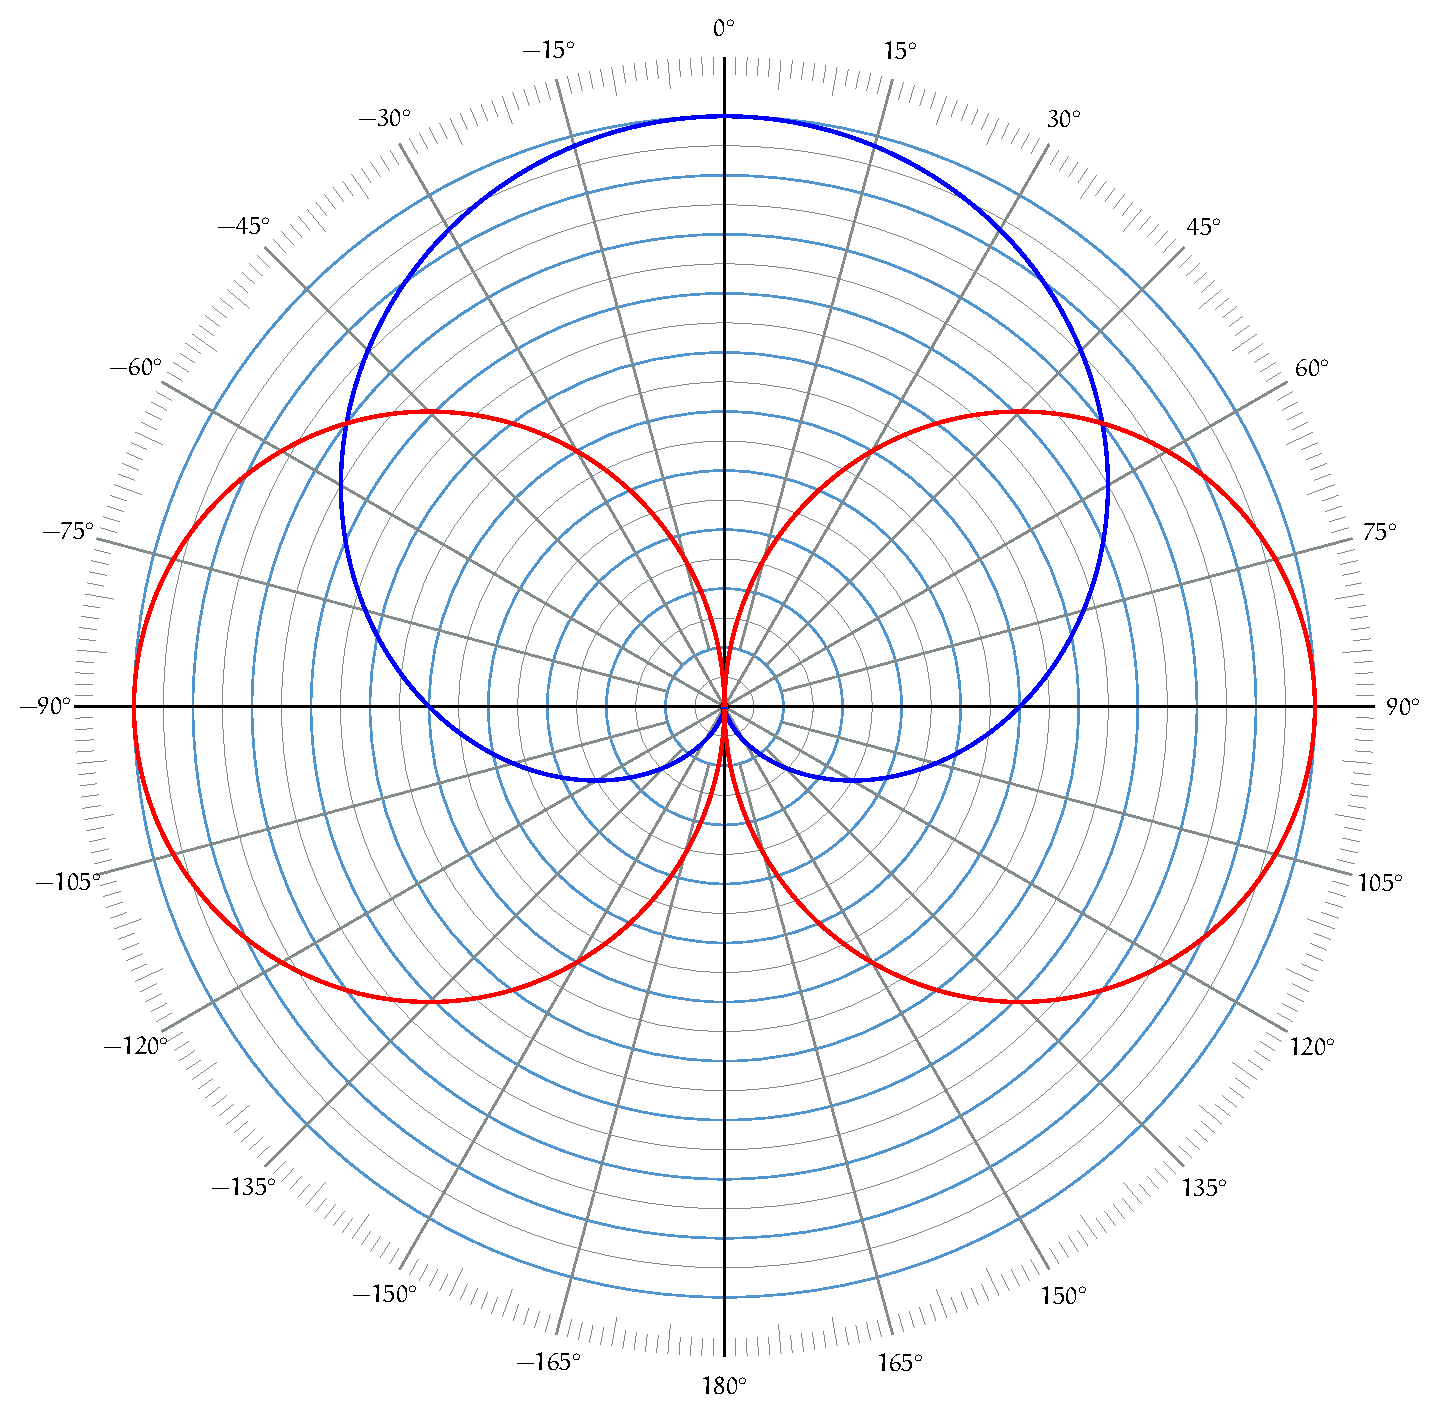
\includegraphics[width=0.99\columnwidth]{microphone-polar-patterns/midside}
\caption[]{Rappresentazione ideale della coppia stereofonica Mid-Side costituita da
da un microfono direzionale cardioide a gradiente di pressione mediante la sua
equazione polare: $cpg = 0.5(x) + 0.5(x\cos\theta)$ (\emph{cardioid pressure
gradient}) e da un microfono bidirezionale a gradiente di
pressione mediante la sua equazione polare: $bpg = x\cos\theta$
(\emph{bidirectional pressure gradient}). Nella tecnica microfonica di registrazione
Mid-Side il microfono cardioide convenzionalmente viene registrato nel primo canale,
mentre il segnale del microfono bidirezinale viene registrato nel secondo canale.}
\label{polar:midsidemic}
\end{figure}

La produzione di un segnale \emph{Mid-Side} come quello in uscita dalla matrice
somma e sottrazione può essere ottenuta dal posizionamento diretto di una coppia
di microfoni aventi caratteristiche polari adeguate. Il segnale \emph{Mid} è
generalmente prodotto da un microfono direzionale cardioide puntato verso il fronte
stereofonico, mentre il segnale \emph{Side} è generato da un microfono
bidirezionale puntato lateralmente, offrendo al fronte il punto di massimo
annullamento. I due microfoni devono essere allineati verticalmente in modo da
risultare orizzontalmente coincidenti.


%%%%%%%%%%%%%%%%%%%%%%%%%%%%%%%%%%%%%%%%%%%%%%%%%%%%%%%%%%%%%%%%%%%% SECTION SIX
%%%%%%%%%%%%%%%%%%%%%%%%%%%%%%%%%%%%%%%%%%%%%%%%%%%%%%%%%%%%%%%%%%%%%%%%%%%%%%%%
\subsection{Mid-Side \emph{panner}}
\label{subsec:mspanner}

La coppia stereofonica di segnali \emph{Mid-Side} è stata descritta finora come
risultante della matrice somma e sottrazione applicata ad un segnale stereofonico
oppure come segnale prodotto da una coppia di microfoni aventi caratteristiche
oppurtune. Analizziamo ora un terzo sistema in grado di generare una coppia
\emph{Mid-Side} attraverso un sistema di panning.

Il canale frontale \emph{Mid} è comunemente descritto da un microfono cardioide.
Sappiamo che la componente cardioide, come moltre altre figure polari, può
essere risultante da una combinazine misurata di
componenti non-direzionale e bidirezionale.

\begin{equation}
m(x,p,\theta) = (p*x) + ((1-p)*(x\cos\theta)
\label{eq:mid}
\end{equation}

Dove $x$ è il segnale di ingresso, $p$ è il coefficiente di ampiezza che regola
il rapporto di peso tra le due componenti, $0.5$ per ottenere la figura polare
cardioide, $\theta$ è la direzione di impatto angolare espressa in radianti.

La componente \emph{Side} è costituita dalla sola componente bidirezionale.

\begin{equation}
s(x,\theta) = x*(sin(\theta))
\label{eq:side}
\end{equation}

Il codice \emph{Faust} per la costruzione di un \emph{Mid-Side Panner} è
molto simile alle equazioni che descrivono le due figure polari.

%--------------------------------------------
%----------------larghezza massima del codice
\begin{lstlisting}
mspan(x,p,rad) = m,s
with{
  m = (p*x)+((1-p)*(x*cos(rad)));
  s = x*(sin(-rad));
};
\end{lstlisting}

I due segnali in uscita dal panner non possono essere inviati direttamente ad un
sistema di ascolto basato sui due canali sinistra-destra, devono necessariamente
passarli attraverso la matrice somma e differenza ottenere ciò che Blumlein
descrive come la differenza di ampiezza nei segnali degli altoparlanti
ottenuta dalle differenze di fase.

% %--------------------------------------------
% %----------------larghezza massima del codice
% \begin{lstlisting}
% mspan_lr(x,p,rad) = mspan(x,p,rad) : sdmx;
% \end{lstlisting}

\begin{figure}[t]
\centering
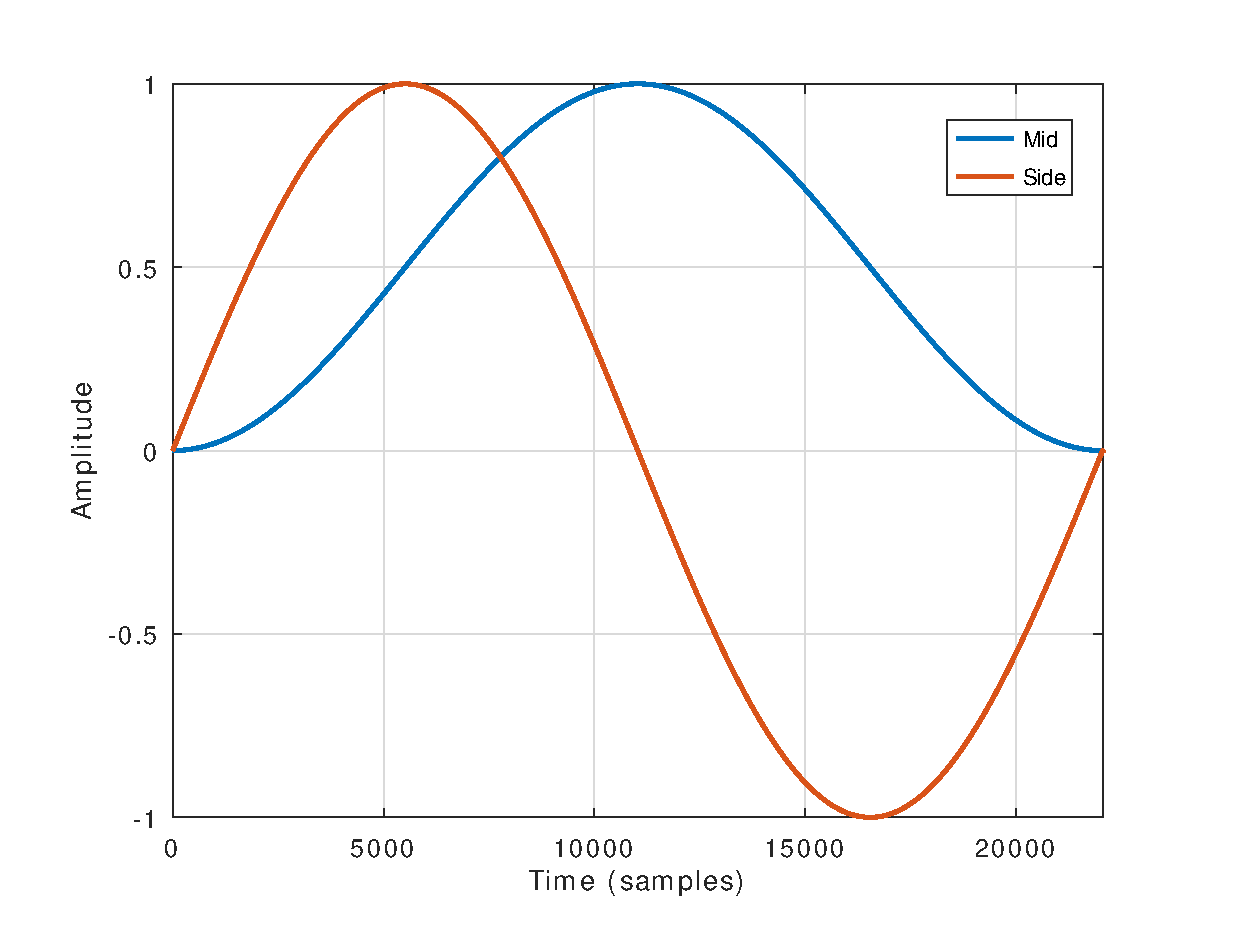
\includegraphics[width=0.99\columnwidth]{CAPITOLI/0300/IMG/mspan}
\caption[]{Mid-Side \emph{panner}. Il grafico mostra la risposta del \emph{panner} ad una
variazione di 360 gradi da sinistra (-180 gradi) a destra (180 gradi). La linea
rossa mostra la bipolarità del segnale correlata alle informazioni angolari. La
linea blu descrive variazioni di ampiezza (sempre con fase positiva) in
relazione alle informazioni angolari. Il grafico mostra l'evidenza della percezione
zero su entrambi gli estremi $\pm180$ gradi, dove cardioide e figura-8 si annullano.}
\label{fig:mspan}
\end{figure}

% La procedura di costruzione dell'algoritmo del \emph{Mid-Side Panner} è completa.
% Il seguente codice di \emph{Faust} descrivo il panner completo di interfaccia
% grafica.

%-----------------------------------------------------------
%-------------------------------larghezza massima del codice
\begin{lstlisting}
//----------------------------------- DEGREES TO RADIANS ---
deg2rad = *(ma.PI/180);
//----------------------------------------------- PANPOT ---
rad = vslider("[02]Azimuth[style:knob]", 0,-180,180,0.1) :
      deg2rad : si.smoo;
//--------------------------------------------- P FACTOR --–
p = vslider("[01]P[style:knob]", 0.5,0,1,0.01) : si.smoo;
//--------------------------------------------- MID-SIDE --–
midside(x,p,rad) = m,s
  with{
    m = (p*x)+((1-p)*(x*cos(rad)));
    s = x*(sin(-rad));
};
//-------------------------------- MS MATRIX DESCRIPTION ---
nsum = 0.5*(_+_);
ndif = 0.5*(_-_);
sdmx = _,_ <: nsum, ndif;
//----------------------------------------- MS2LR MATRIX ---
mspan_lr(x,p,rad) = midside(x,p,rad) : sdmx;
process = os.osc(1000), p, rad : mspan_lr;
\end{lstlisting}


\section{Stereo Pairs}

\begin{quote}
Pur sottolineando l’estrema varietà di combinazioni possibili nell’uso dei
microfoni, sia per registrare che per amplificare, è di fondamentale importanza
un’analisi delle varie configurazioni di coppie stereofoniche perché,
soprattutto nel campo della registrazione, esse possono, e molto spesso devono,
essere considerate come il punto di partenza per l’installazione di un set-up
di registrazione.
\end{quote}

Così \index[names]{Schiavoni, Piero} Piero Schiavoni iniziava le sue lezioni
sulle coppie stereofoniche al Conservatorio S. Cecilia di Roma. Questo tipo di
ragionnamento ci riporta al principio di questo percorso sulla stereofonia:
la fisiologia dell'ascolto umano e le motivazioni del suono riprodotto.

Come chiarito da Blumlein \cite{ab58} fin dal principio, l'ascolto binaurale umano
oltre a riferire al cervello del mondo acustico circostante, sono in grado di
fornire le informazioni necessarie alla ricostruzione tridimensionale di tale
mondo.


Naturalmente, per quanto possano
essere tecnologicamente avanzati, i microfoni non potranno neanche lontanamente
eguagliare la perfezione dell’udito umano, che si avvale di qualche millennio
di “affinamento” evolutivo, nondimeno un corretto uso delle varie tecniche di
ripresa stereofonica è il mezzo per portarci quanto più vicino possibile al
lavoro compiuto internamente dal nostro apparato uditivo.

Attraverso una buona tecnica di ripresa stereofonica è possibile ricostruire nel
nostro cervello un’immagine sonora che si avvicini alla percezione reale, e
trasmettere nel miglior modo possibile il contenuto culturale ed emozionale
dell’evento musicale. Occorre inoltre tenere ben presente che il giudizio finale
dell’orecchio dipende in gran misura dal sistema di ascolto della registrazione,
per cui un ascolto effettuato con cuffia avrà una resa sensibilmente diversa d
quello effettuato con diffusori, per problemi ben precisi di psicoacustica, di
cui accenneremo in seguito. Il sistema di ascolto di riferimento è generalmente
quello con diffusori, in cui il punto di ascolto, naturalmente centrale rispetto
alla coppia di altoparlanti, è situato al vertice di un angolo di sessanta gradi.

\subsection{Parametri di valutazione}

Una ripresa stereofonica può essere valutata sotto diversi aspetti, ognuno dei
quali costituisce, nell'osservazione della stereofonia, un parametro d’ascolto:

\begin{compactitem}
\item localizzazione
\item definizione timbrica
\item profondità
\item spaziosità
\end{compactitem}

\begin{figure}[th]
\centering
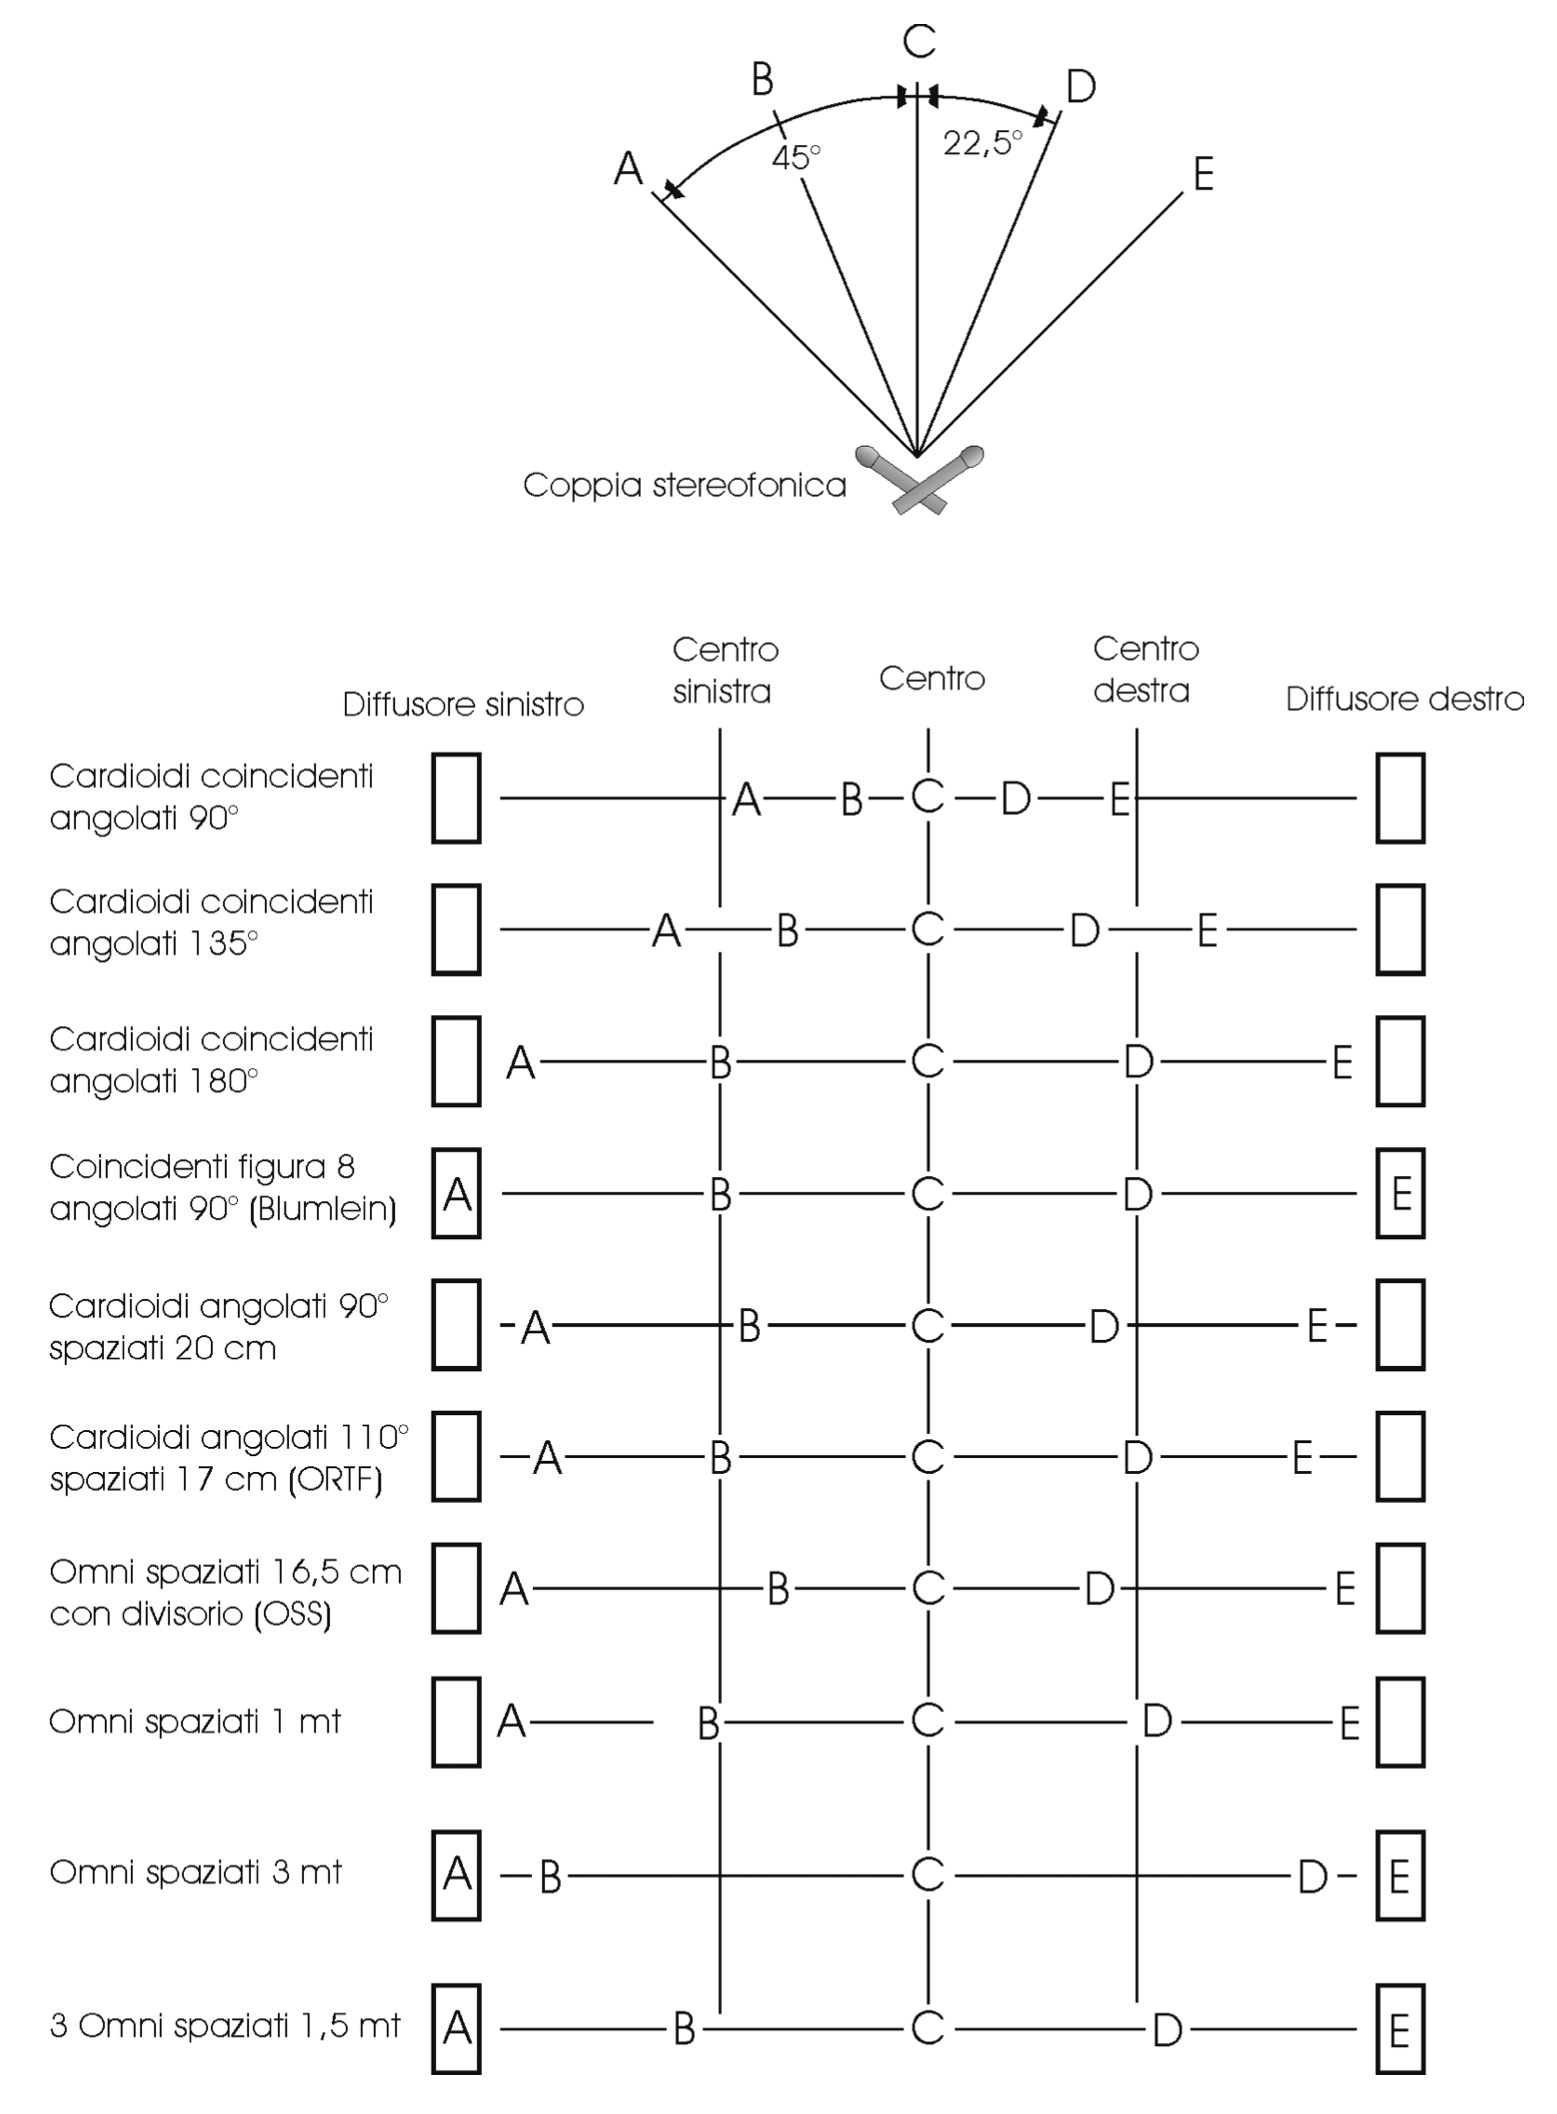
\includegraphics[width=0.99\columnwidth]{CAPITOLI/0300/IMG/localizzazione}
\caption[]{Ripresa di un fronte sonoro e localizzazione}
\label{fig:localizzazione}
\end{figure}

\subsection{Localizzazione}

La localizzazione è la capacità della ripresa di riprodurre una posizione degli
strumenti nello spazio orizzontale (da sinistra a destra) che si avvicini il più
possibile a quella originaria. Nella fig. \ref{fig:localizzazione} vediamo nella
parte superiore una coppia che riprende un fronte sonoro ipotetico di $90°$, e
in questo fronte sono evidenziati, oltre agli estremi (A e E), alcuni punti
intermedi (centro-sinistra B, centro C e centro-destra D). Nella parte inferiore
a differenti tecniche di ripresa, corrispondono differenti risultati di
percezione della localizzazione attraverso il riascolto con un sistema
stereofonico di diffusori: alcuni di questi si avvicinano in modo soddisfacente
alla riproduzione della posizione originaria, altri (ad es. la coppia coincidente
angolata di 90°) denotano una riproduzione ristretta, tendente a centrare i
suoni, altri (ad es. la coppia omni spaziata di 3 mt.) presentano, all’opposto,
una separazione eccessiva tra i canali ed un conseguente “buco” nel centro
d’ascolto.

\subsection{La definizione timbrica}

La definizione timbrica è dovuta in gran parte alla capacità di riprodurre la
gamma di frequenze originaria senza coloriture e senza perdite. Dando per
scontato l’utilizzo di microfoni professionali in cui l’accuratezza della
risposta in frequenza sia di livello adeguato, bisogna notare che il risultato
relativo a questo parametro dipende da diversi fattori: dalla caratteristica
polare del microfono stesso, dall’angolazione tra questo e la fonte sonora, e
dalla possibile influenza delle riflessioni dovute all’ambiente che possono, per
effetti di cancellazione di fase, alterare la risposta in frequenza del microfono
producendo colorazioni e buchi nella linearità della stessa.

\subsection{La profondità}

La profondità della ripresa non è altro se non la possibilità di distinguere,
all’interno del gruppo orchestrale, differenti piani sonori, come è nella realtà,
per cui gli archi devono risultare in un piano più ravvicinato rispetto ai legni,
collocati immediatamente alle spalle dei primi, e questi devono essere a loro
volta collocati davanti agli ottoni e alle percussioni. Naturalmente eventuali
solisti avranno la precedenza nei confronti della massa orchestrale, a meno che,
come nel caso delle riprese di opere liriche, si desideri mantenere il rapporto
scenico, con le voci più lontane rispetto all’orchestra. In mancanza della
definizione di questa dimensione, il problema può essere quello di un appiattimento
dell’orchestra su un piano orizzontale, con il risultato di una ripresa, magari
buona dal punto di vista degli altri parametri, ma poco interessante e coinvolgente.

\subsection{La spaziosità}

La spaziosità della ripresa consiste nella capacità di riproduzione dell’ambiente
in cui si effettua la ripresa, quindi una registrazione che voglia tener conto
di questo parametro conterrà una certa dose del riverbero ambientale presente
nella sala. Naturalmente, la misura del riverbero ambientale dovrà essere dosata,
oltre che dall’esperienza e dal gusto, dall’attenzione che deve essere posta nell
salvaguardia della definizione timbrica dello strumento. Anche qui, il risultato
dipenderà da diversi fattori: l’acustica della sala innanzitutto, e poi la scelta
della configurazione, nonché il posizionamento della coppia stessa. Un
posizionamento molto vicino allo strumento (o al gruppo orchestrale) darà un
rapporto suono diretto/suono riverberato più favorevole al suono diretto, rispetto
ad un posizionamento della coppia ad una certa distanza.

\subsection{Tipologie di coppie stereofoniche}

Entrando più in dettaglio sulle tipologie di configurazione, e partendo dal
presupposto di avere a disposizione due microfoni della stessa marca e dello stesso
modello e con caratteristiche simili (risposta in frequenza, curva polare, ecc.),
possiamo dividere le coppie in tre categorie:

\begin{compactitem}
\item coppie coincidenti
\item coppie quasi-coincidenti
\item coppie spaziate
\end{compactitem}

\subsection{Coincidenti}

Le coppie coincidenti, comunemente note come XY, consistono in due microfoni i
cui diaframmi di ripresa siano esattamente sovrapposti, in una vista ortogonale
dall’alto, una volta posti di fronte alla sorgente sonora. Una caratteristica
comune a tutte le coppie coincidenti è che offrono in assoluto la migliore
compatibilità mono, vale a dire che nel momento in cui si vadano a sommare i du
canali si hanno i minori fenomeni di cancellazione dovuti alle differenze di fase
dei due segnali.

\subsubsection{Blumlein}

Il primo esempio è dato dalla coppia coincidente figura-8 angolata di $90°$,
cioè la cosiddetta configurazione Blumlein, (a cui ci si riferisce come
inventore della stereofonia e di alcune tecniche di ripresa stereofonica). Come
si può vedere nella fig. 3, mentre il microfono corrispondente al canal
sinistro prende la parte sinistra dell’orchestra, per effetto della configurazione
a 8 prende anche l’ambiente retrostante destro, e inversamente farà l’altro canale.
Concettualmente, questa configurazione può essere pensata anche per quello che
ciascuno dei microfoni non prende (il sinistro non prende nulla del lato destro
dell’orchestra, coincidente col punto di annullamento massimo, e ugualmente
l’altro canale). Questa configurazione rimane una delle più precise come
equilibrio tra tutti i parametri sopra descritti.

Nella configurazione Blumlein è importante che il “fronte sonoro” sia contenuto
nell’apertura a 90° della coppia, per evitare l’influenza degli spostamenti di
fase dovuti al suono catturato dai microfoni nelle rispettive zone retrostanti.

\subsubsection{XY}

Usando due cardioidi in coppia coincidente, è possibile variare la loro
angolatura, così avremo una coppia angolata a $180°$, che darà una buona
localizzazione, a scapito di una scarsa definizione nella zona centrale,
dovuta al fenomeno per cui i suoni fuori-asse si attenuano nelle componenti più
acute, ed è una configurazione da tenere presente nel caso il fronte sonoro
sia limitato in ampiezza e si desideri avere una grande apertura sul
riverbero ambientale.

Angolando i microfoni a $135°$, avremo un miglioramento
della definizione, perché le curve polari, riducendo l’angolatura, tendono
sommare le risposte. Questa coppia ha una minore apertura stereo, è può essere
utilizzata quando si voglia raggiungere questo risultato.

Riducendo ancora l’angolatura, abbiamo la coppia angolata a $90°$ che, come
evidenziato nella tabella di fig. \ref{fig:localizzazione}, è la configurazione
che presenta la più ridotta apertura stereo, tendendo a concentrare i suoni
verso il centro. Può essere desiderabile quando il fronte sonoro è molto ampio
e si sia obbligati a riprenderlo molto da vicino.

\clearpage

\begin{figure*}[t]
    \centering
    \begin{subfigure}[t]{0.99\textwidth}
        \centering
        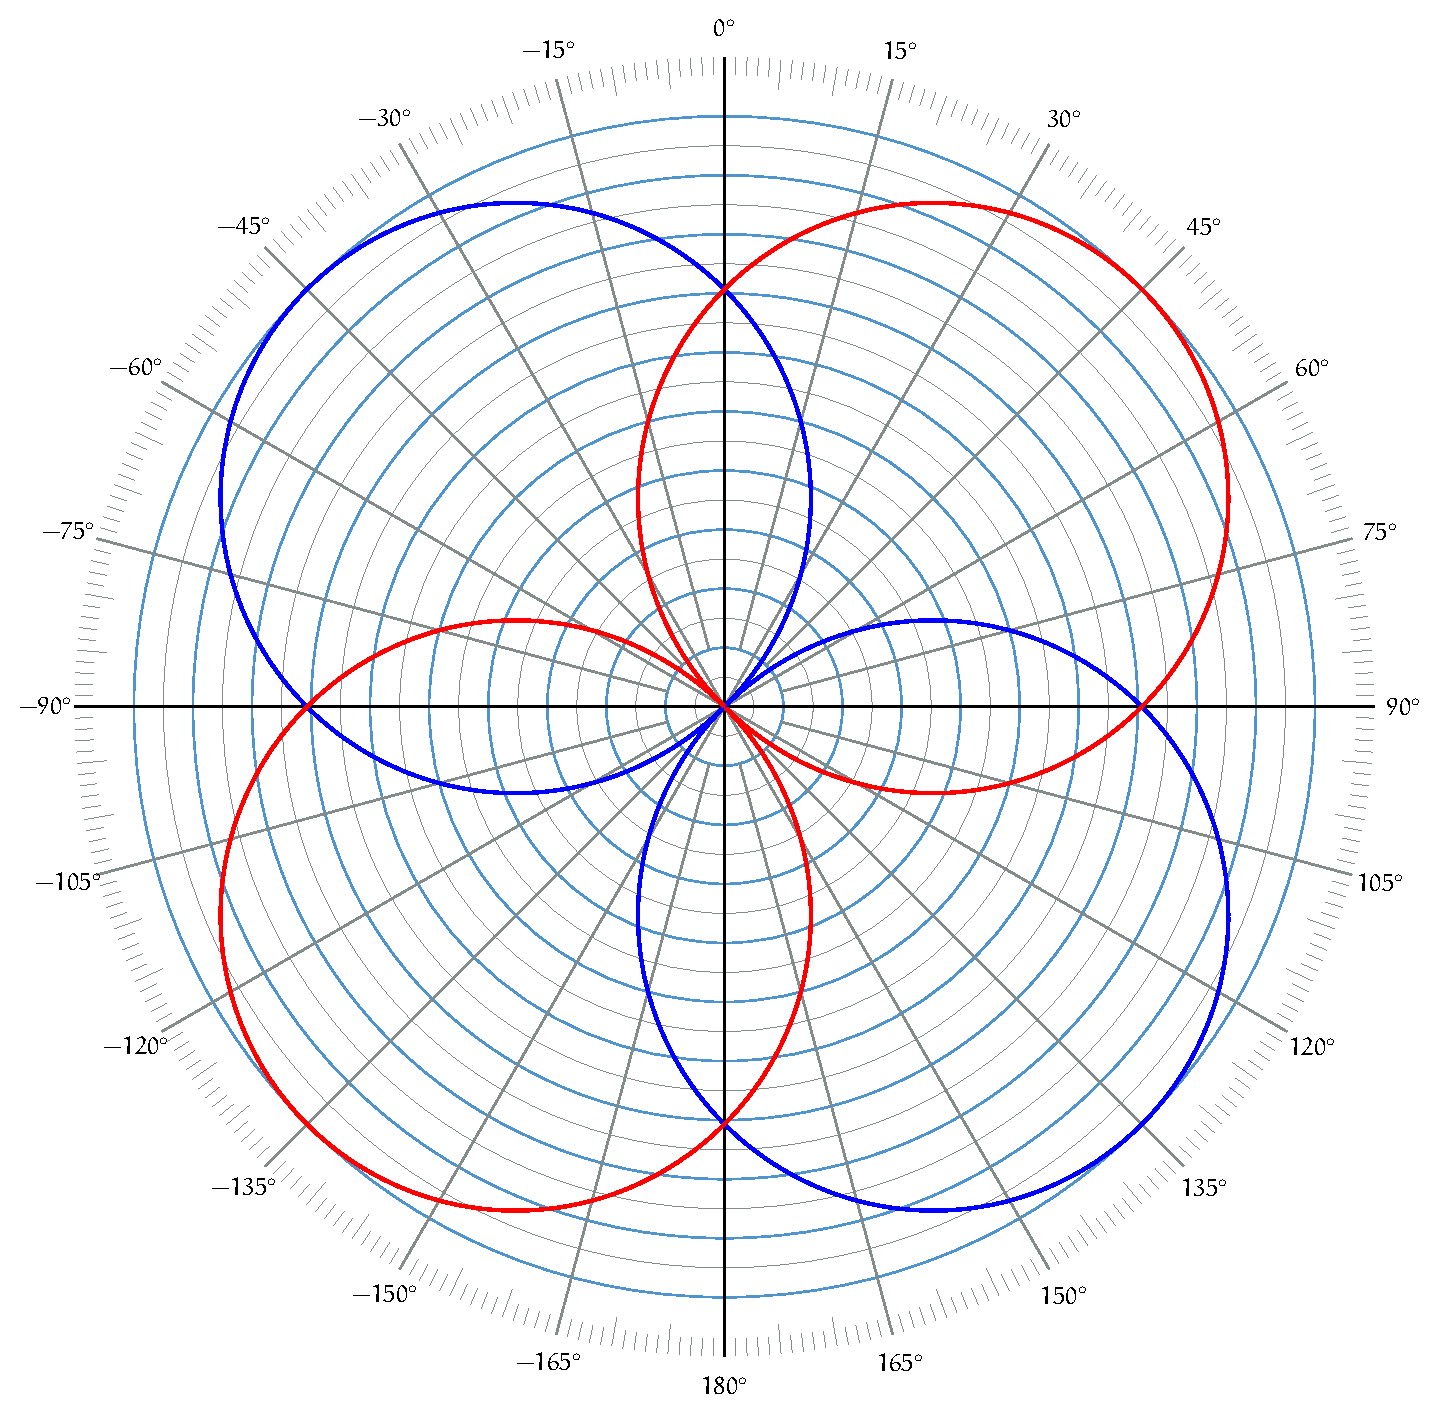
\includegraphics[width=11cm]{microphone-polar-patterns/blumlein}
        \caption[]{BLUMLEIN. Coppia stereofonica coincidente di figura-8 angolati tra loro di $90°$.}% \\ Eq: $1(x)$}
        \label{pol:blumleinsp}
    \end{subfigure}%
    \\
    \begin{subfigure}[t]{0.99\textwidth}
        \centering
        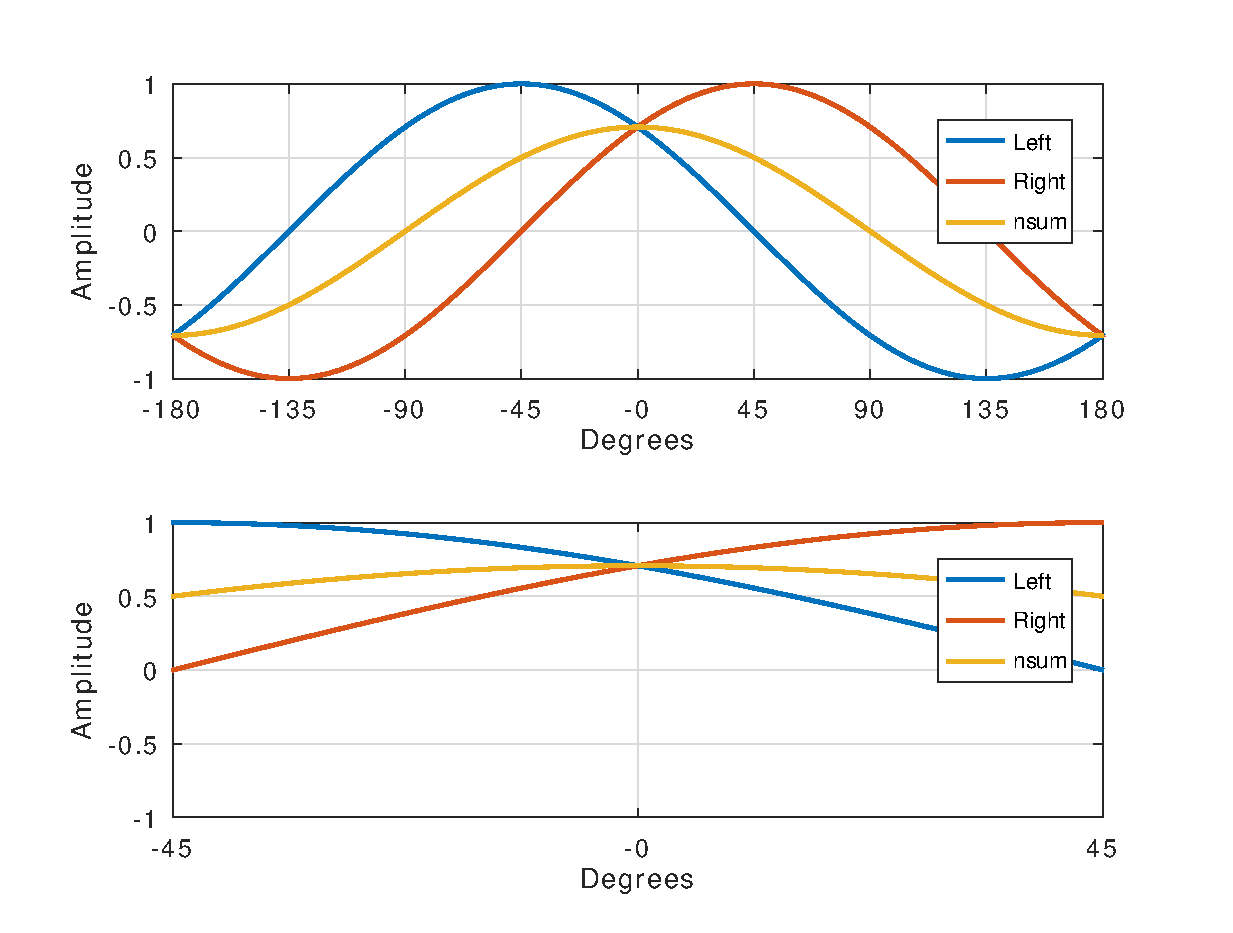
\includegraphics[width=12.5cm]{CAPITOLI/0300/IMG/blumleinsub}
        \caption[]{Variazioni angolari di ampiezza.}% \\ Eq: $0.75(x)+0.25(x\cos\theta)$}
        \label{plot:blumlein}
    \end{subfigure}
    \caption[]{BLUMLEIN}
    \label{sp:blumlein}
\end{figure*}

\clearpage

\begin{figure*}[t]
    \centering
    \begin{subfigure}[t]{0.99\textwidth}
        \centering
        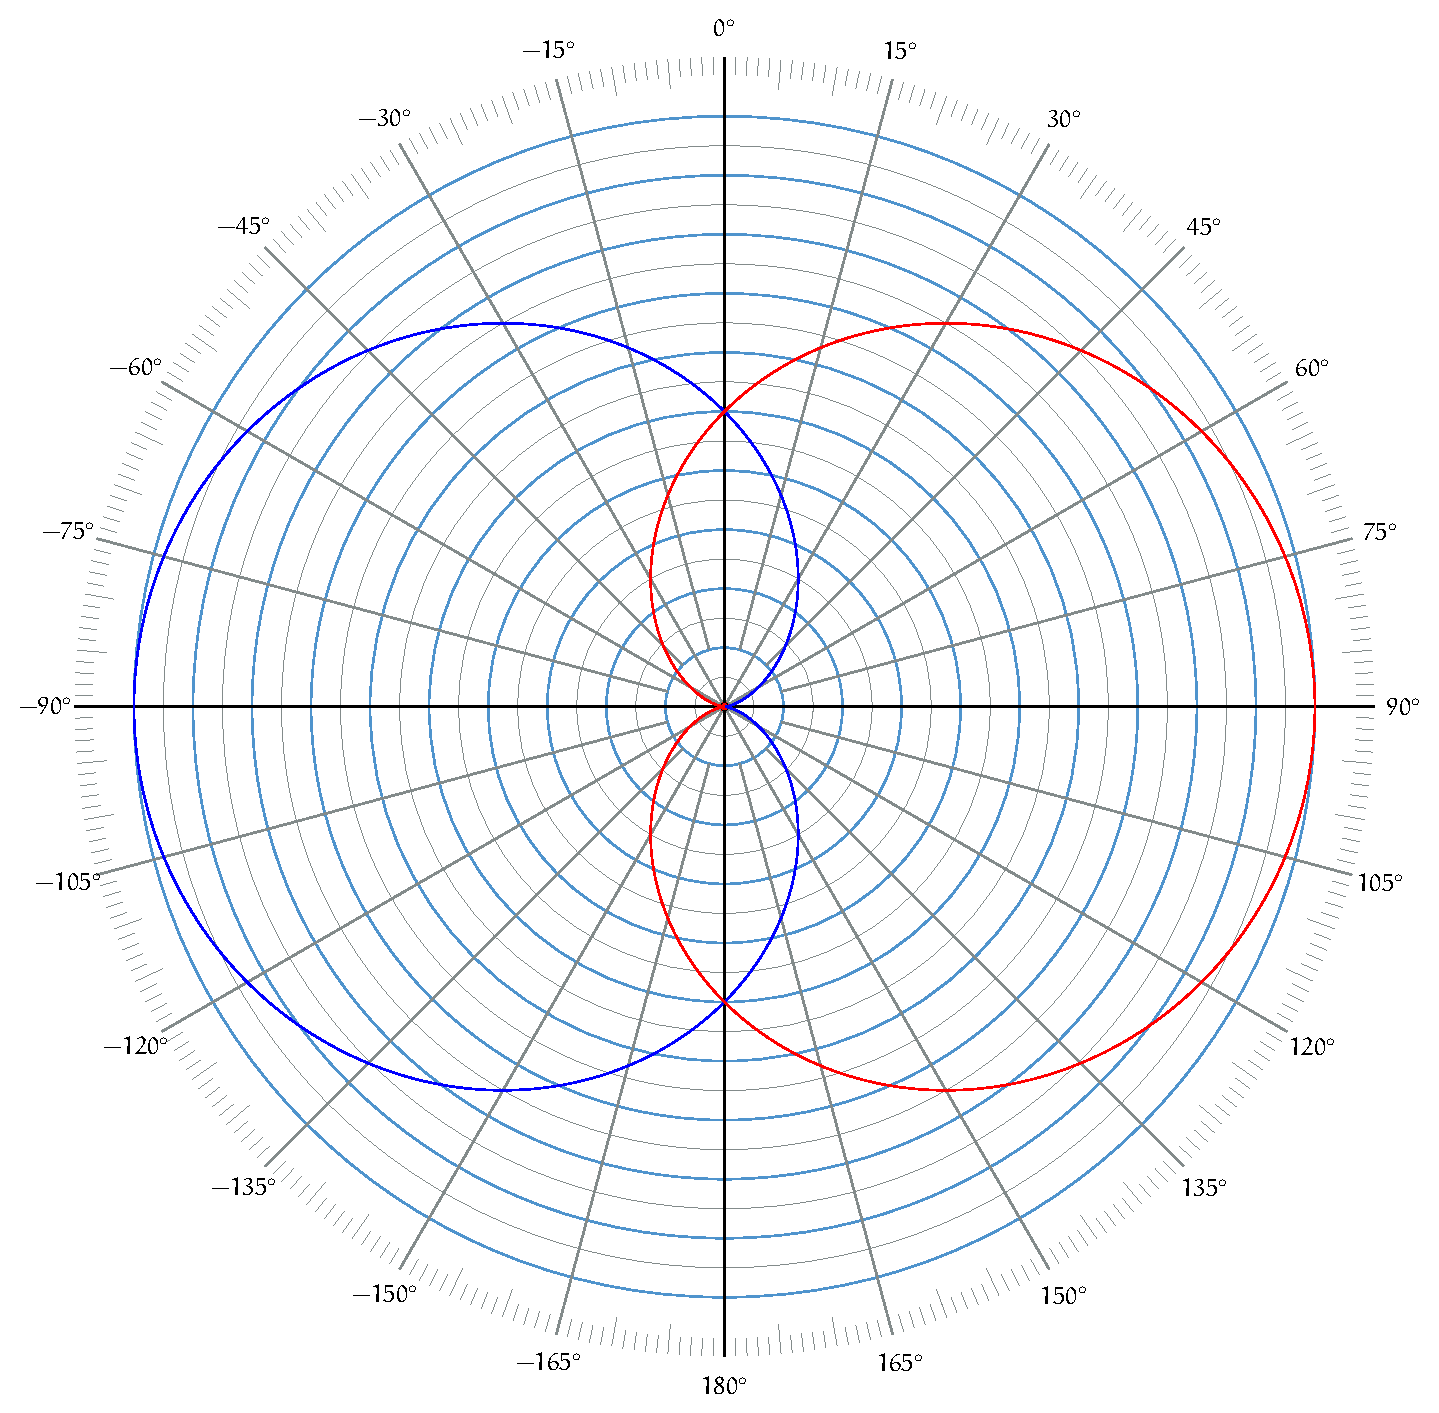
\includegraphics[width=11cm]{microphone-polar-patterns/xy180}
        \caption[]{XY90. Coppia stereofonica coincidente di cardioidi angolati tra loro di $180°$.}% \\ Eq: $1(x)$}
        \label{pol:xy120sp}
    \end{subfigure}%
    \\
    \begin{subfigure}[t]{0.99\textwidth}
        \centering
        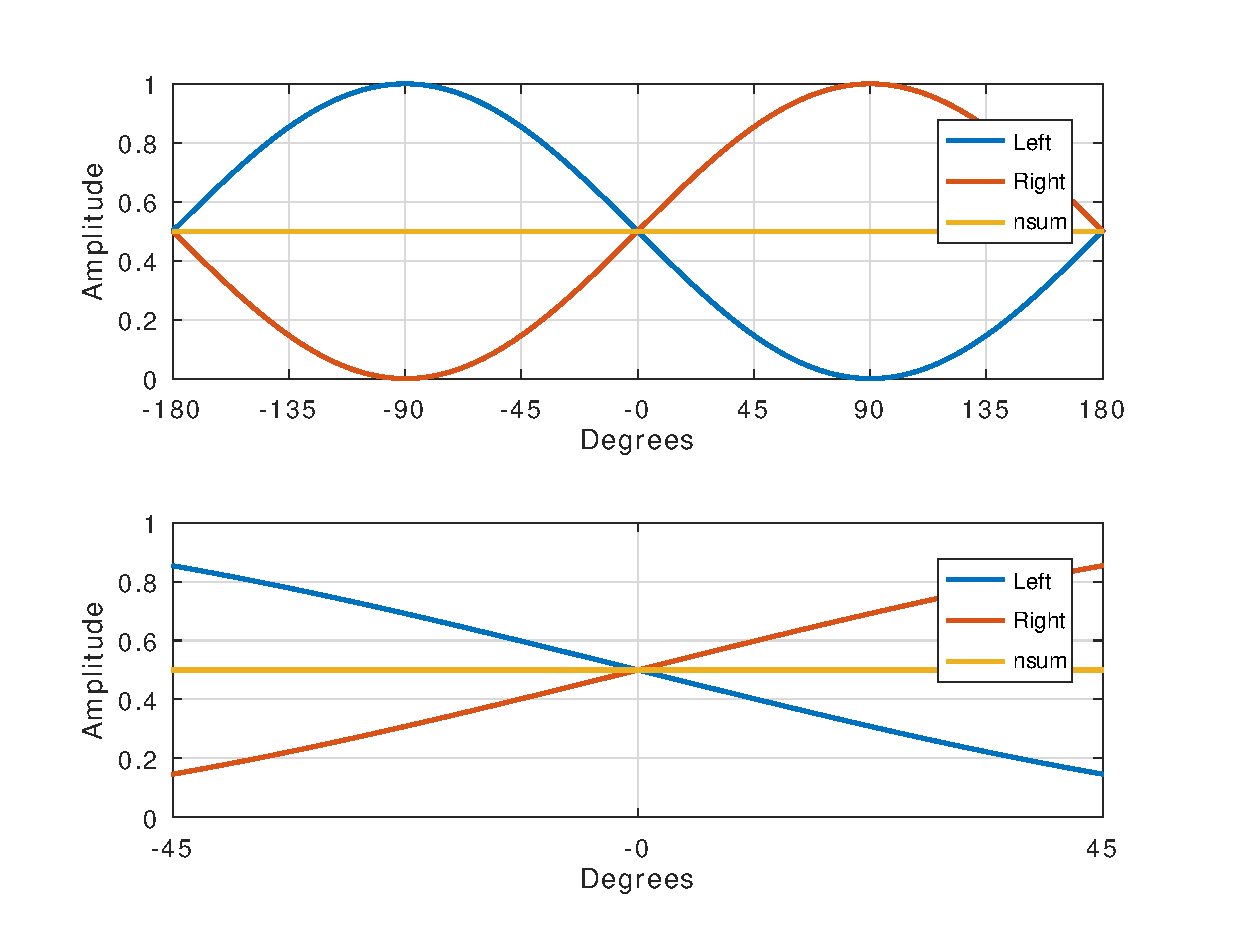
\includegraphics[width=12.5cm]{CAPITOLI/0300/IMG/xy180sub}
        \caption[]{Variazioni angolari di ampiezza.}% \\ Eq: $0.75(x)+0.25(x\cos\theta)$}
        \label{plot:xy180}
    \end{subfigure}
    \caption[]{XY180}
    \label{sp:xy180}
\end{figure*}

\clearpage

\begin{figure*}[t]
    \centering
    \begin{subfigure}[t]{0.99\textwidth}
        \centering
        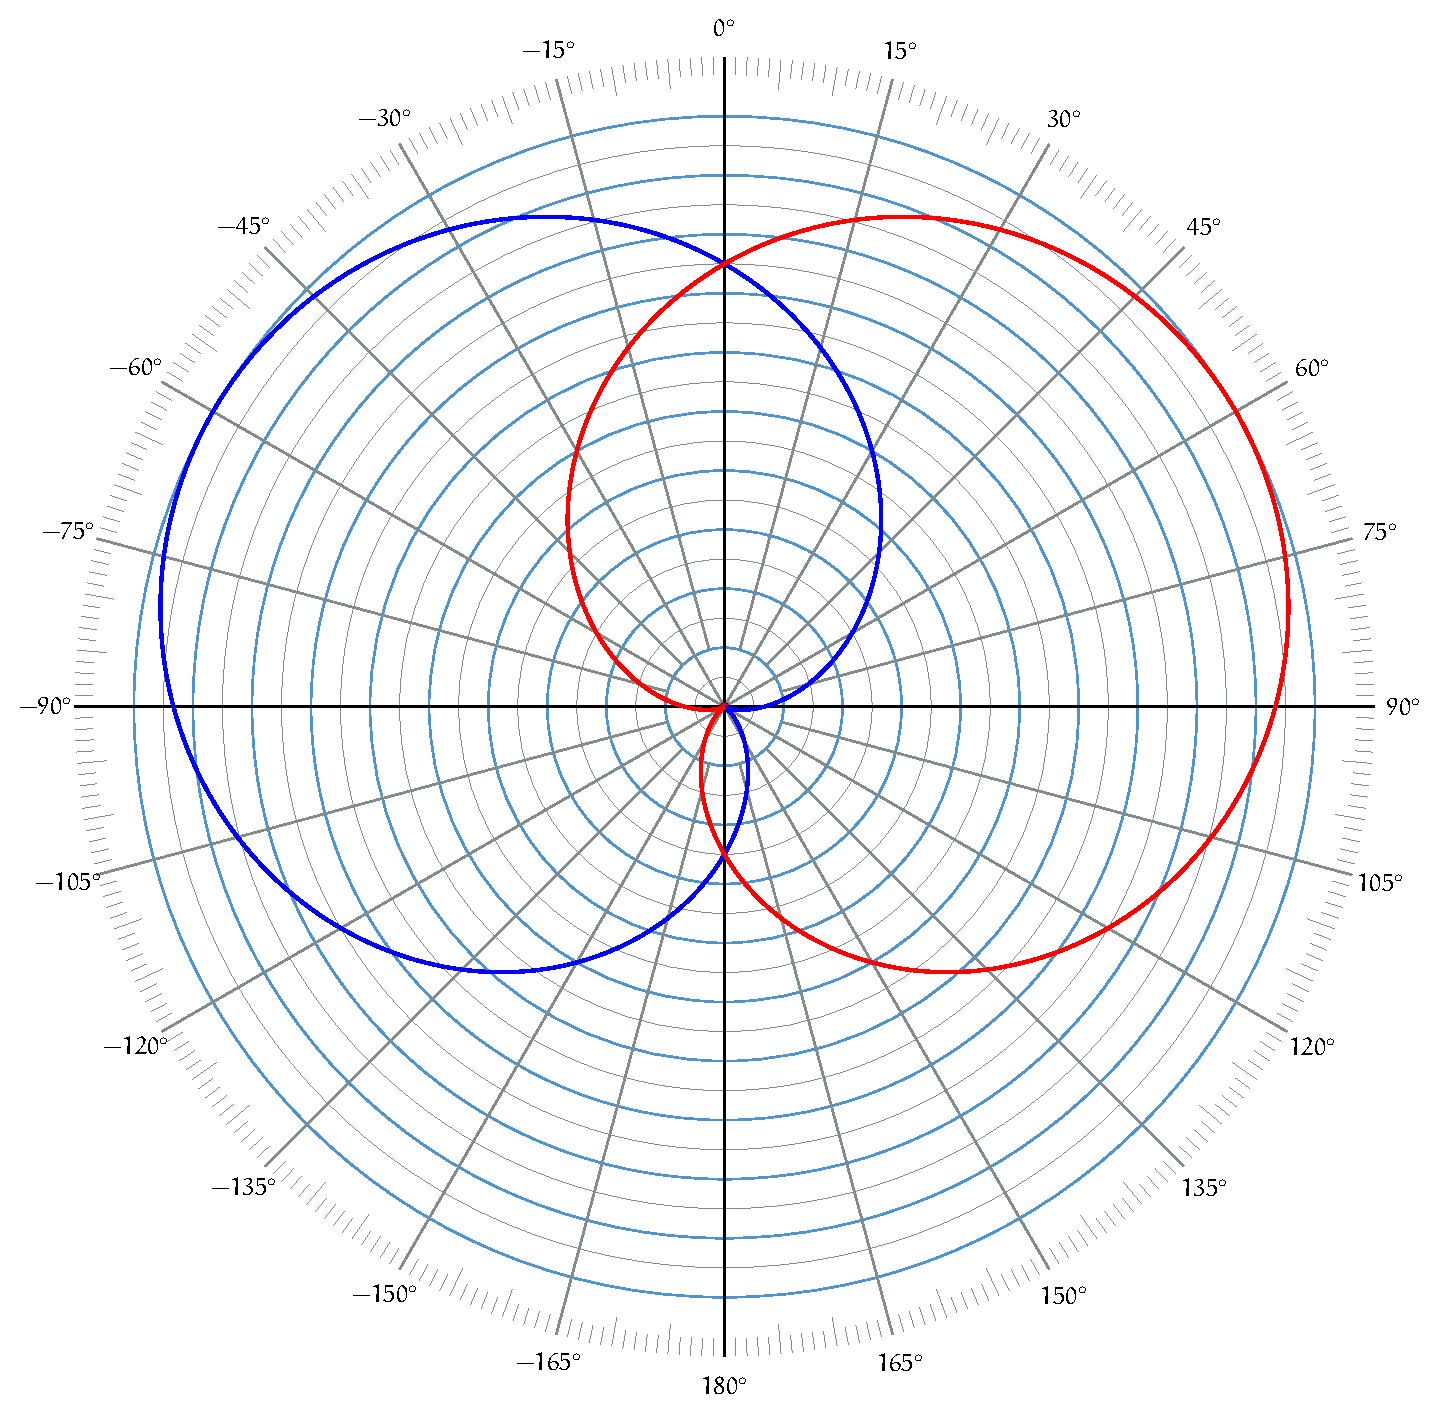
\includegraphics[width=11cm]{microphone-polar-patterns/xy120}
        \caption[]{XY90. Coppia stereofonica coincidente di cardioidi angolati tra loro di $120°$.}% \\ Eq: $1(x)$}
        \label{pol:xy120sp}
    \end{subfigure}%
    \\
    \begin{subfigure}[t]{0.99\textwidth}
        \centering
        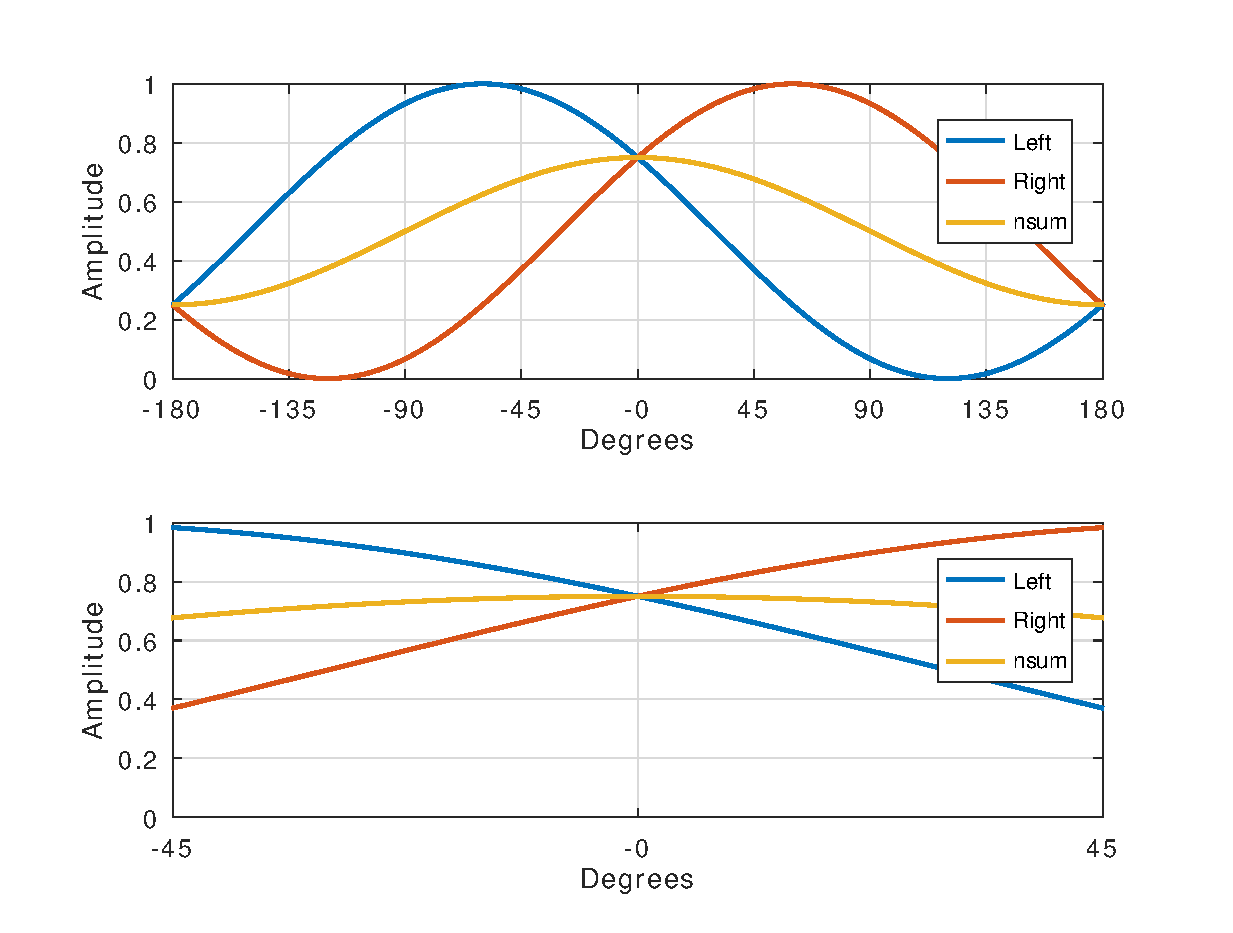
\includegraphics[width=12.5cm]{CAPITOLI/0300/IMG/xy120sub}
        \caption[]{Variazioni angolari di ampiezza.}% \\ Eq: $0.75(x)+0.25(x\cos\theta)$}
        \label{plot:xy120}
    \end{subfigure}
    \caption[]{XY120}
    \label{sp:xy120}
\end{figure*}

\clearpage

\begin{figure*}[t]
    \centering
    \begin{subfigure}[t]{0.99\textwidth}
        \centering
        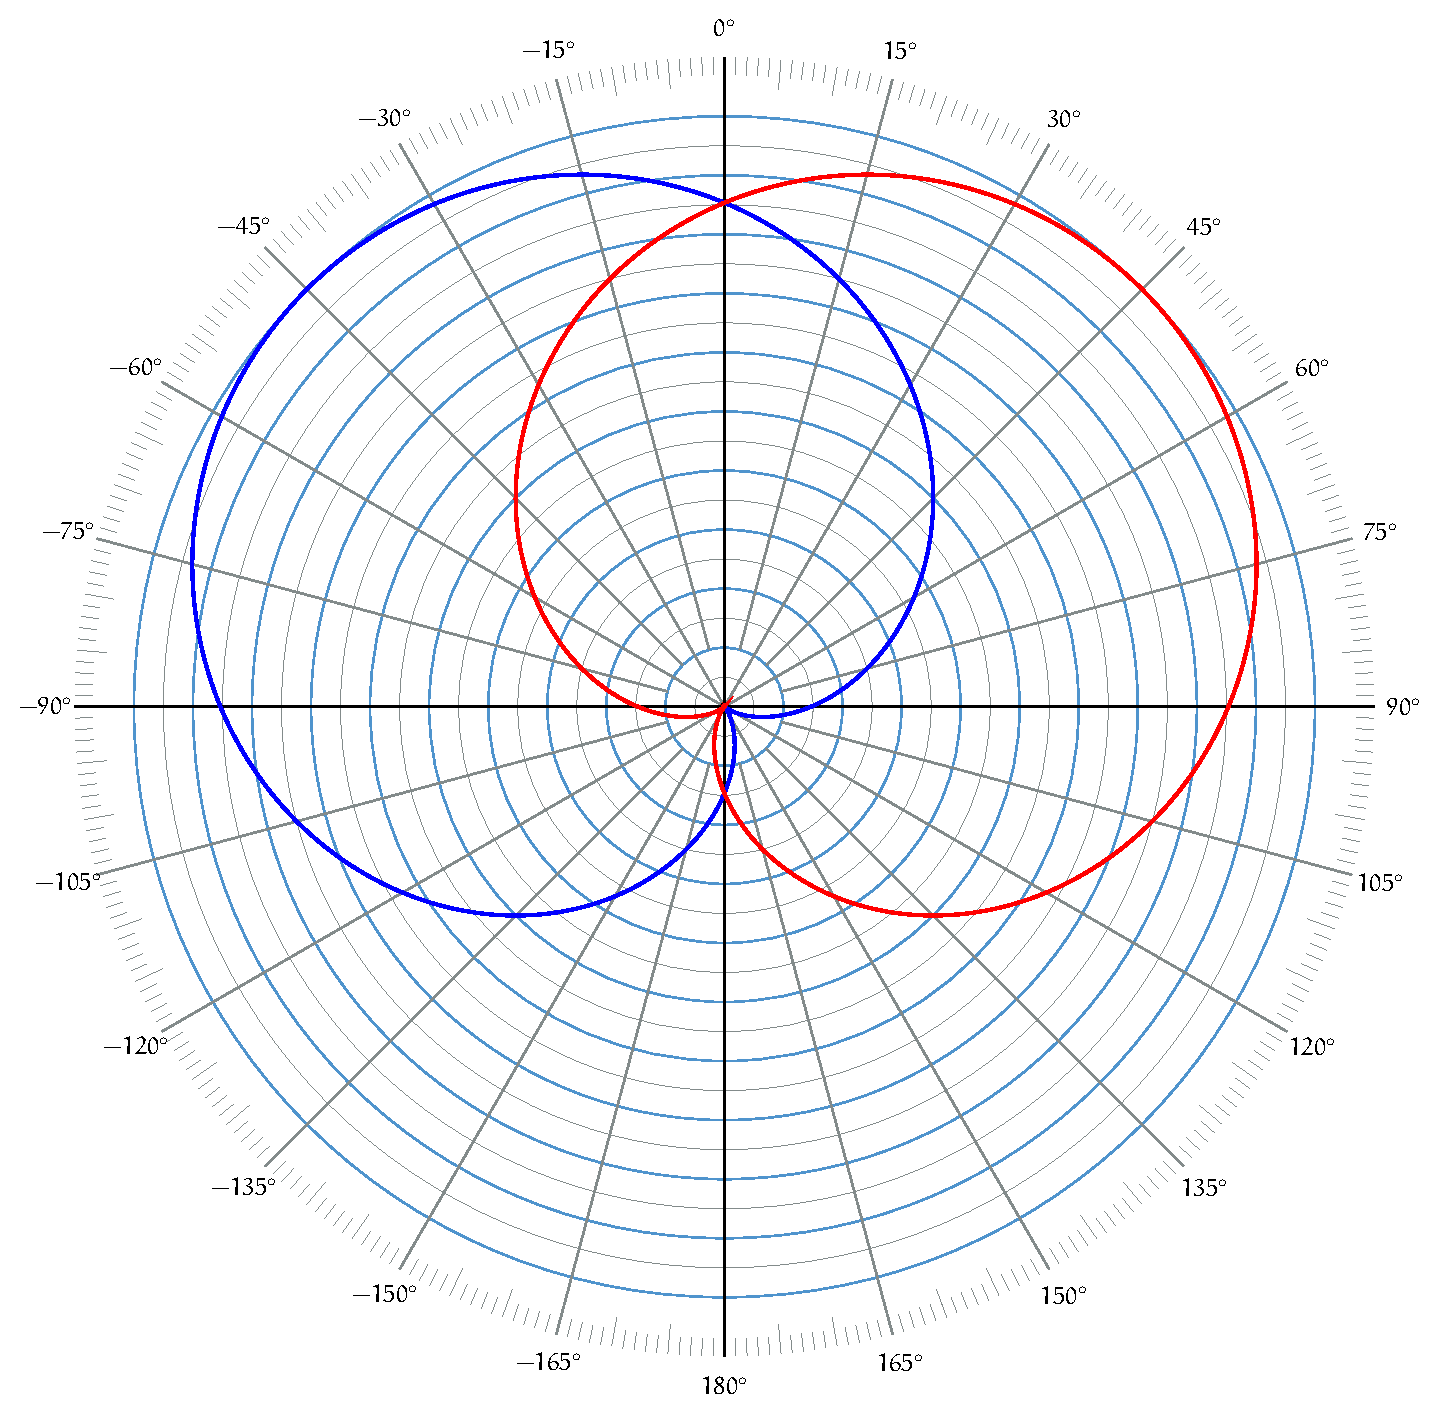
\includegraphics[width=11cm]{microphone-polar-patterns/xy90}
        \caption[]{XY90. Coppia stereofonica coincidente di cardioidi angolati tra loro di $90°$.}% \\ Eq: $1(x)$}
        \label{pol:xy90sp}
    \end{subfigure}%
    \\
    \begin{subfigure}[t]{0.99\textwidth}
        \centering
        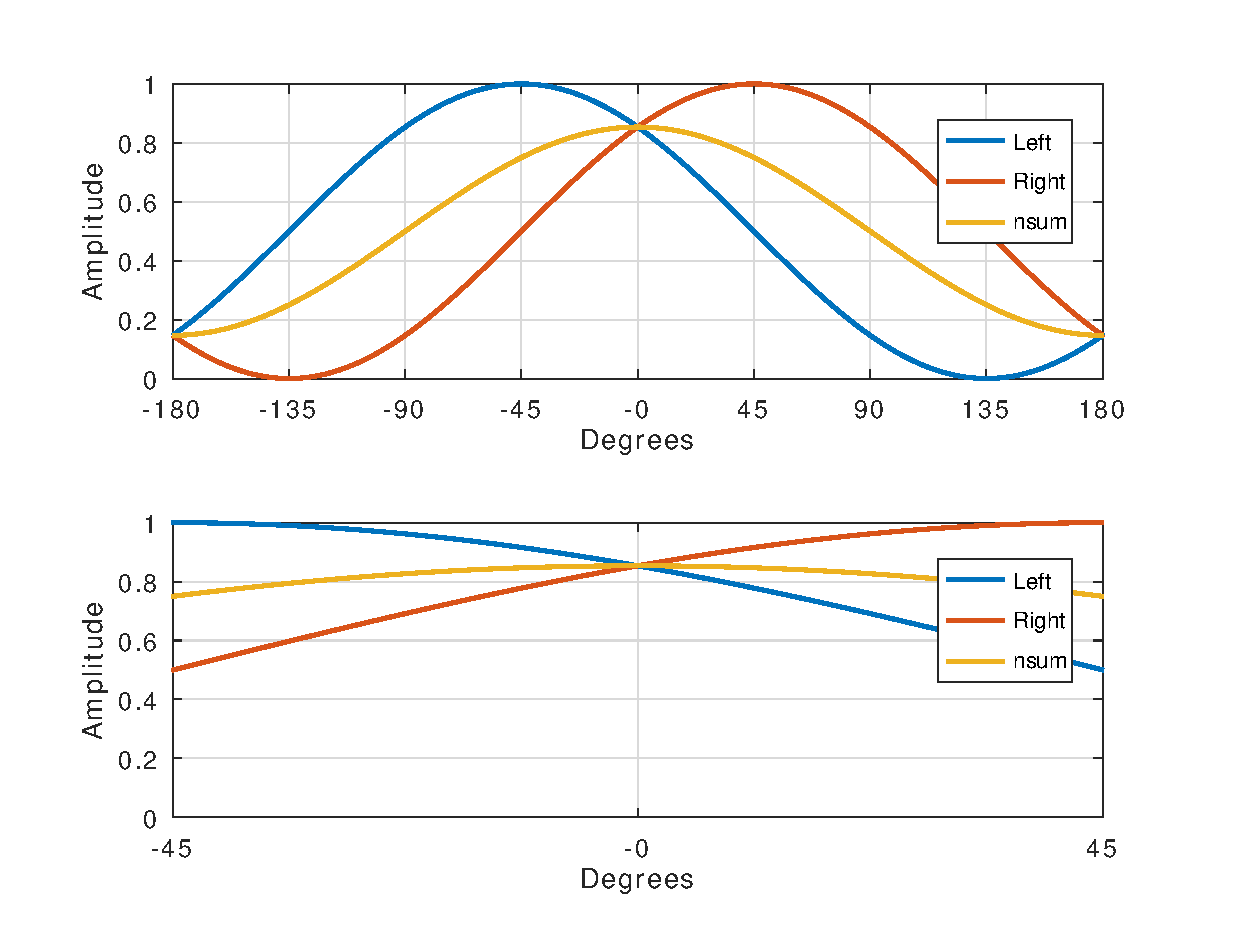
\includegraphics[width=12.5cm]{CAPITOLI/0300/IMG/xy90sub}
        \caption[]{Variazioni angolari di ampiezza.}% \\ Eq: $0.75(x)+0.25(x\cos\theta)$}
        \label{plot:xy90}
    \end{subfigure}
    \caption[]{XY90}
    \label{sp:xy90}
\end{figure*}

\clearpage

\subsection{Semi-coincidenti}

Le coppie quasi-coincidenti, rispetto a quelle esaminate fin qua, offrono una
maggiore ampiezza di immagine stereofonica ed una resa più ricca della riverberazione
ambientale. Per converso, diminuisce la compatibilità mono, in quanto allontanando
tra loro i diaframmi dei microfoni diminuisce la coerenza di fase, in special
modo alle alte frequenze.

Nella fig. \ref{pol:ortfsp} è illustrata una coppia angolata di $110°$ e spaziata
di $17cm$, la cosiddetta coppia ORTF, dal nome dell’allora ente radiotelevisivo
francese all’interno del quale è stata sviluppata. Può essere considerata i
assoluto come una delle migliori soluzioni per tutti i parametri sopra illustrati.

Un’altra coppia quasi-coincidente, la configurazione “DIN”, dove l’angolatura
è stata ridotta a 90° e la distanza tra le capsule portata a 20 cm. Come si può
constatare dalla tabella di fig. \ref{fig:localizzazione}, questo porta a
spostare verso il centro i suoni intermedi e ad allargare i suoni estremi.
Se la distanza viene portata a 30 cm la configurazione prende il nome di “NOS”.

\clearpage

\begin{figure*}[t]
    \centering
    \begin{subfigure}[t]{0.99\textwidth}
        \centering
        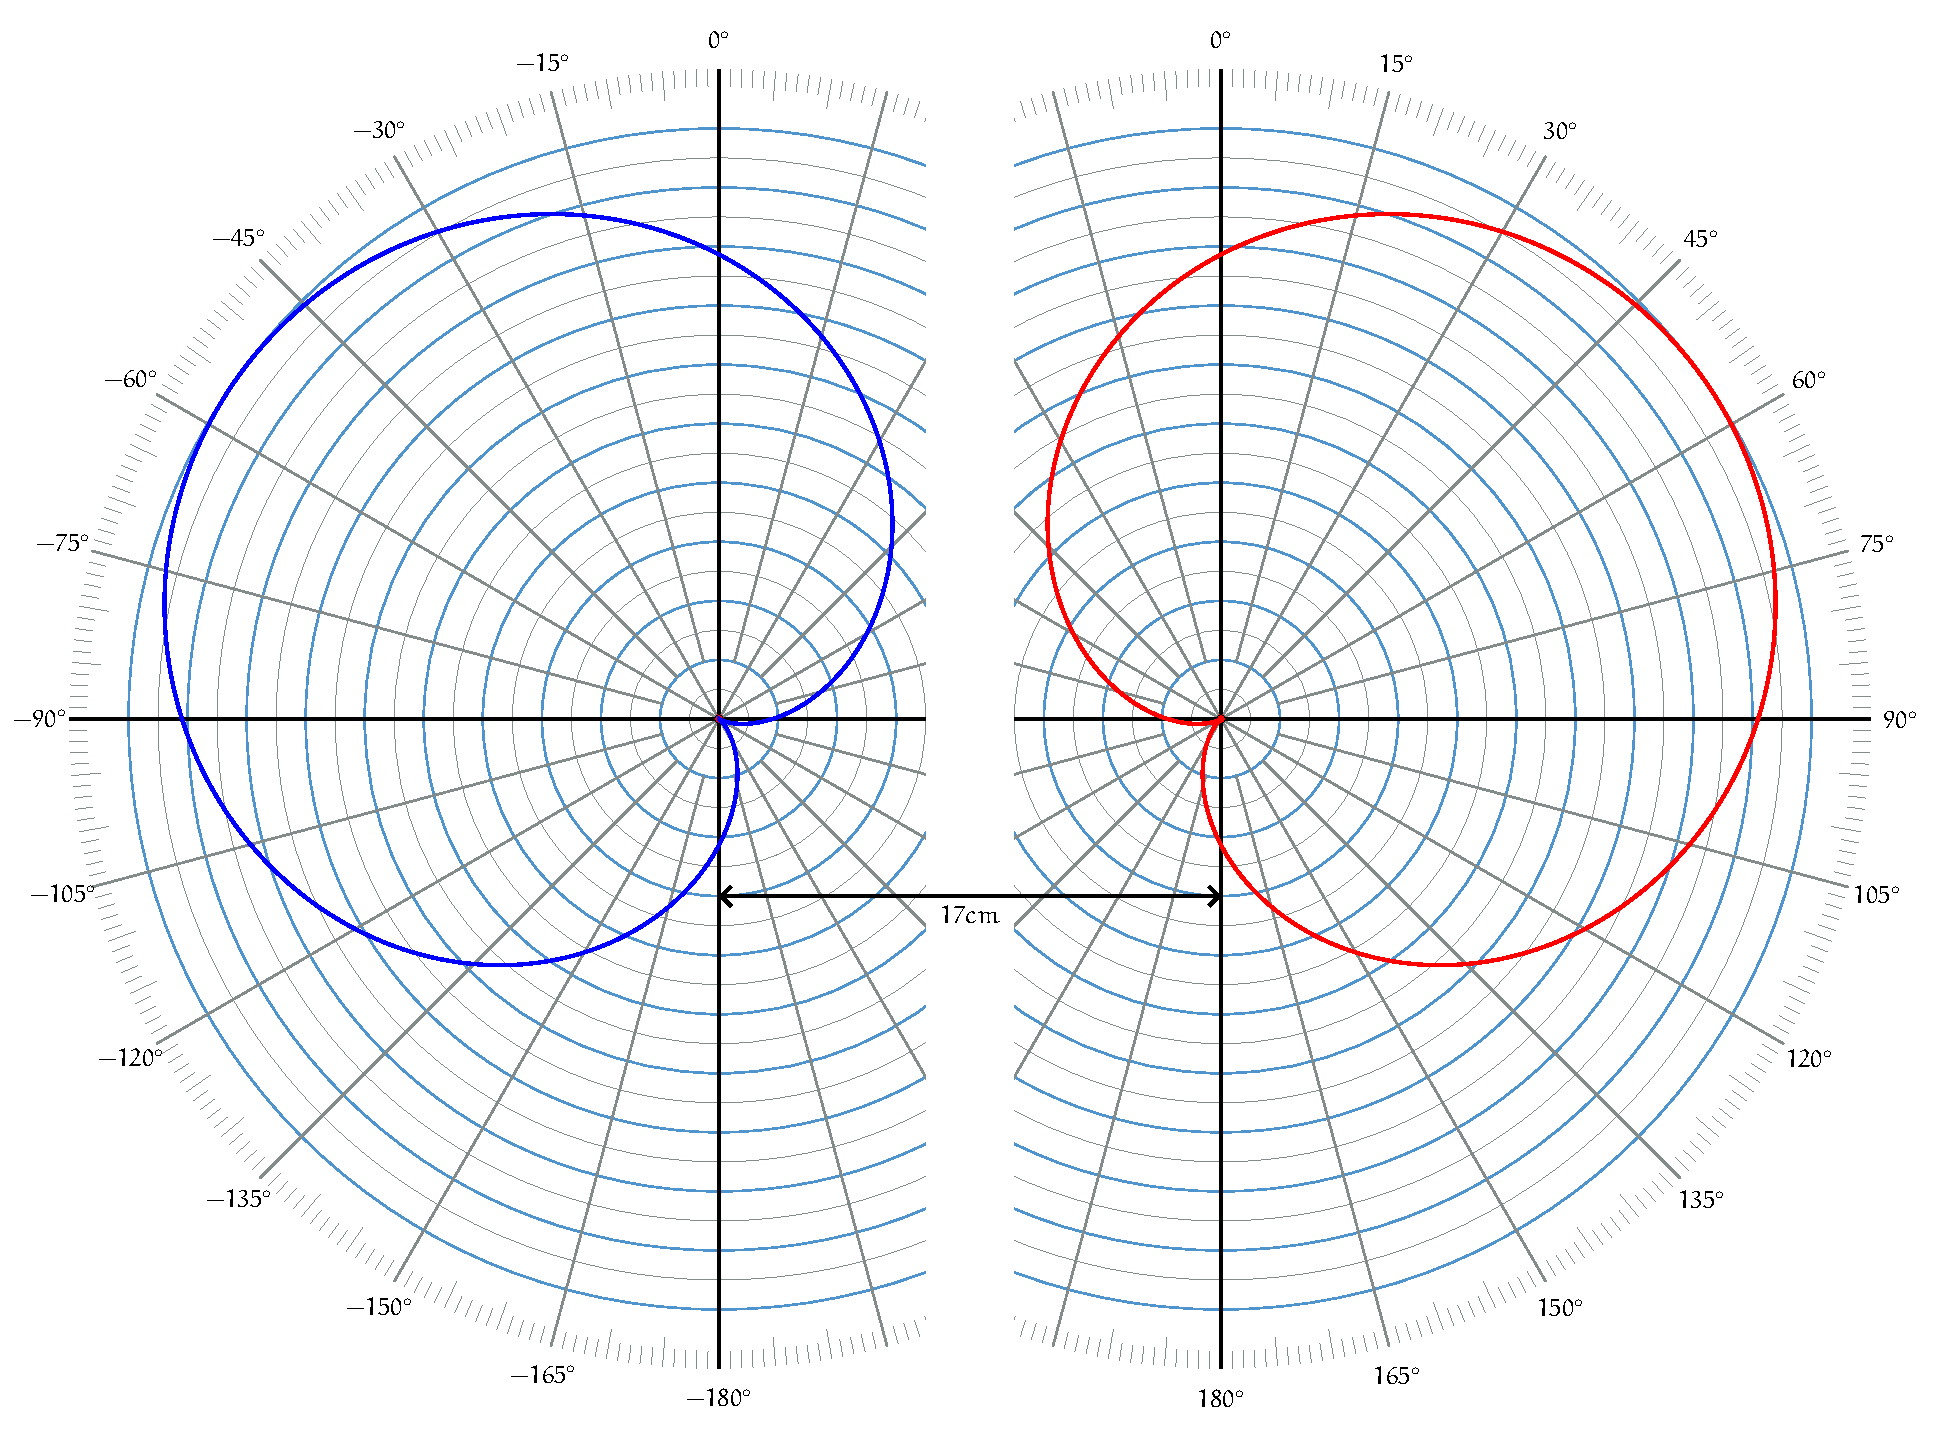
\includegraphics[width=11cm]{microphone-polar-patterns/ORTF}
        \caption[]{ORTF. Coppia stereofonica semi-coincidente di cardioidi angolati tra loro di $110°$ e distanti $17cm$.}% \\ Eq: $1(x)$}
        \label{pol:ortfsp}
    \end{subfigure}%
    \\
    \begin{subfigure}[t]{0.99\textwidth}
        \centering
        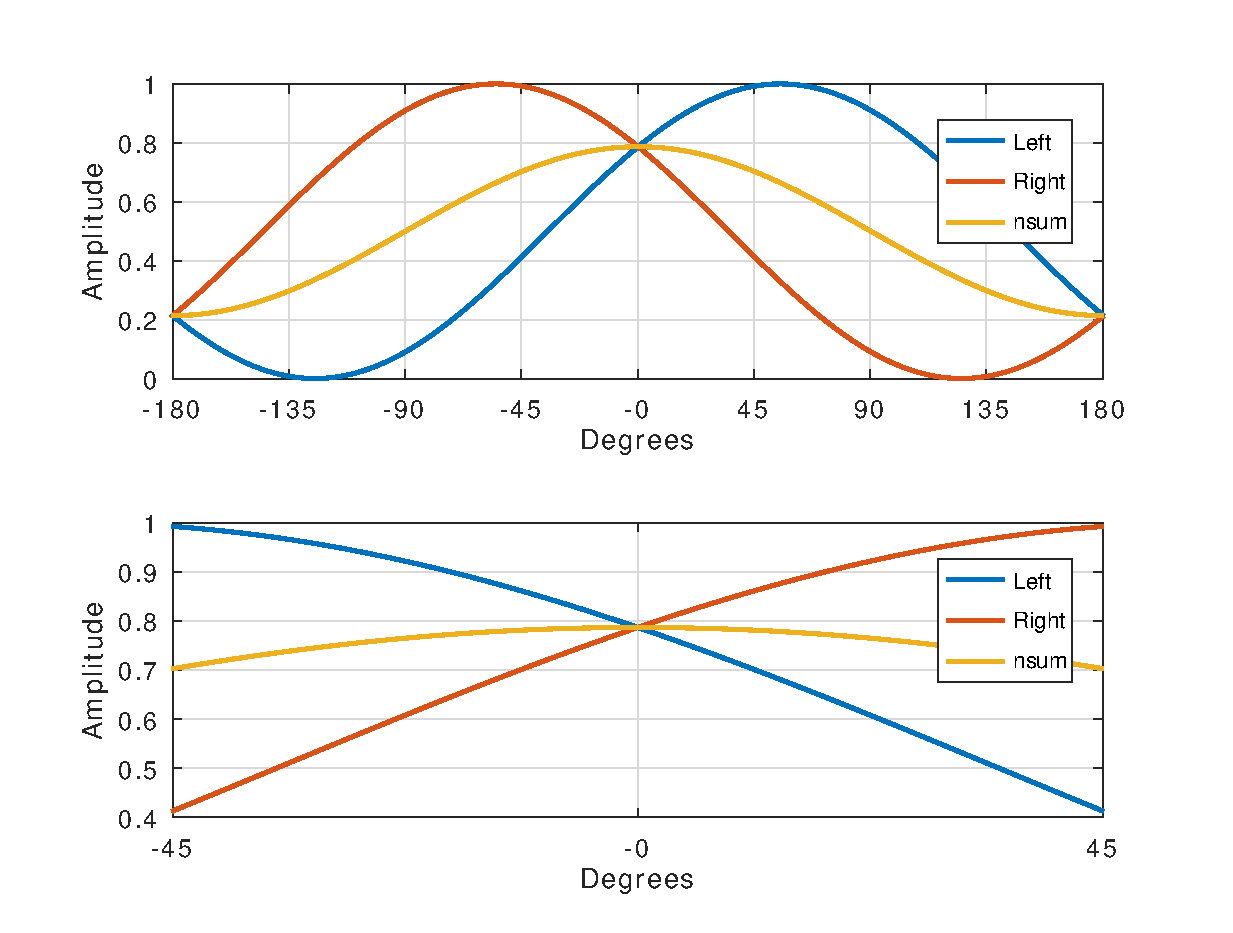
\includegraphics[width=12.5cm]{CAPITOLI/0300/IMG/ortfsub}
        \caption[]{Variazioni angolari di ampiezza.}% \\ Eq: $0.75(x)+0.25(x\cos\theta)$}
        \label{plot:ortf}
    \end{subfigure}
    \caption[]{ORTF}
    \label{sp:ortf}
\end{figure*}

\clearpage

\subsection{Le coppie spaziate}

Le coppie spaziate sono generalmente costituite da microfoni omnidirezionali
posizionati in parallelo tra di loro, rivolti verso la fonte sonora, e spaziati
di una certa distanza. Essendo entrambi i microfoni orientati nella stessa
direzione senza angolatura, la stereofonia è data dalla diversità di tempo
con cui il suono raggiunge i due microfoni, che si traduce anche in una
differenza di fase. E’ un tipo di ripresa molto adatto in ambienti dove il
riverbero ambientale è molto equilibrato, come ad es. un auditorium, in
quanto la capsula omnidirezionale riesce a restituire con ricchezza di dettaglio
anche gran parte del suono fuori asse. Altra caratteristica importante del
microfono omnidirezionale è la capacità di ripresa dei suoni gravi, superiore
a quella dei microfoni direttivi, per cui, nel caso di una registrazione
orchestrale, potrà rendere in maniera migliore suoni che si estendono molto
nella gamma bassa, come i contrabbassi, la grancassa, ecc. Va detto che tra
tutte le configurazioni è quella con la minor compatibilità mono, a causa delle
differenze di fase sopra descritte, per cui ove fosse impiegata in ripresa che
potrebbero avere un utilizzo in mono (ad es. riprese televisive), va usata con
prudenza e va controllato l’ascolto in mono per essere sicuri che non siano
avvertibili cancellazioni di fase.

%Nella fig. 10 la spaziatura è stata portata a 3 metri, e nella tabella di fig. 2 si può notare la differenza di questa ripresa rispetto alla precedente: gli strumenti tendono ad ammucchiarsi o tutti a sinistra o tutti a destra, lasciando un buco al centro.

%Nella fig. 11 nella configurazione precedente vediamo inserito un microfono centrale, che sul mixer sarà assegnato a entrambi i canali (left-right), con la funzione di ricreare il centro mancante. Questa configurazione, in realtà, non è più una coppia microfonica, essendo i microfoni tre, ma è generalmente considerata una variante delle configurazioni precedenti. In tale configurazione si usano indifferentemente sia microfoni cardioidi che omnidirezionali, e una grande cura deve essere posta nel posizionamento in vista di possibili effetti di “comb-filter” tra i tre microfoni.

Un ulteriore variante dei tre omnidirezionali è il cosiddetto “albero Decca”
(Decca tree), sviluppato dall’omonima casa discografica, dove il microfono
centrale è stato collocato in una posizione molto avanzata, in modo da dare
alla ripresa un centro assolutamente stabile, in conseguenza anche delle
differenze di tempo d’arrivo del suono. Il microfono preferito per questa
configurazione, quello con il quale questa configurazione è nata, è il
Neumann M50, ossia un microfono omnidirezionale a pressione dotato di una marcata
esaltazione delle frequenze alte in asse.

Un interessante configurazione è rappresentata dal sistema OSS (Jecklin disk),
in cui due microfoni omnidirezionali, spaziati di $16.5cm$, sono separati da un
divisorio rigido ricoperto di materiale fonoassorbente. Un tale sistema è vicino
alla simulazione di una testa umana, e può essere utile in riprese destinate
all’ascolto in cuffia (registrazioni binaurali).

Un’importante configurazione è la cosiddetta MS (mid-side), che consiste in un
microfono direzionale (cardioide o ipercardioide) sovrapposto ad un microfono
figura-8 disposto in modo da avere il punto di annullamento massimo in direzione
frontale. In tal modo, il microfono direttivo conterrà l’informazione relativa
al suono centrale (mid), mentre l’altro conterrà l’informazione relativa al
suono laterale (side).

%Il microfono mid entra in un canale e viene inviato, tramite il potenziometro panpot, ad entrambi i canali di uscita, mentre il microfono side viene fatto entrare su due canali, uno dei quali avrà il commutatore di fase invertito. Questi due canali vengono assegnati uno all’uscita sinistra e l’altro all’uscita destra, e potranno essere dosati e controllati tramite i relativi potenziometri del livello (fader). Il vantaggio di questa configurazione risiede proprio nella possibilità di separare l’informazione centrale da quella laterale, e di avere l’opportunità di controllare il bilanciamento di queste due informazioni.

%Un’ultima coppia stereofonica da segnalare è quella nota come “Testa artificiale” (Dummy Head, fig. 16), che consiste in una coppia di microfoni, generalmente omnidirezionali, installati all’interno di una struttura riproducente la conformazione di una testa umana, e posizionati in corrispondenza delle orecchie. Tale configurazione, tendente a simulare nel modo più accurato possibile la percezione umana, produce un tipo di registrazioni note come “registrazioni binaurali”, di cui tratteremo in seguito.

\subsection{Dummy Head}


\printbibliography
\end{refsection}
